\DeclareUnicodeCharacter{2028}{} 
\documentclass{article}
\usepackage[dvipsnames]{xcolor}
\usepackage{listings}
\usepackage{alloy-style}
\usepackage{blindtext}
\usepackage[section]{placeins}
\usepackage[T1]{fontenc}
\usepackage[utf8]{inputenc}
\usepackage{titling}
\usepackage{float}
\usepackage{tikz}
\usetikzlibrary{calc}
\usetikzlibrary{arrows.meta}
\usepackage{graphicx}
\usepackage{hyperref}




\title{ Requirement Analysis and Specification Document\\2020-2021}
\author{Alessandro Polidori (Codice persona 10573078)\\Olimpia Rivera (Codice persona 10617517)}
\date{}



\renewcommand{\contentsname}{Table of Contents}


\begin{document}

\renewcommand{\labelitemi}{\normalfont -}

\begin{figure}[]
  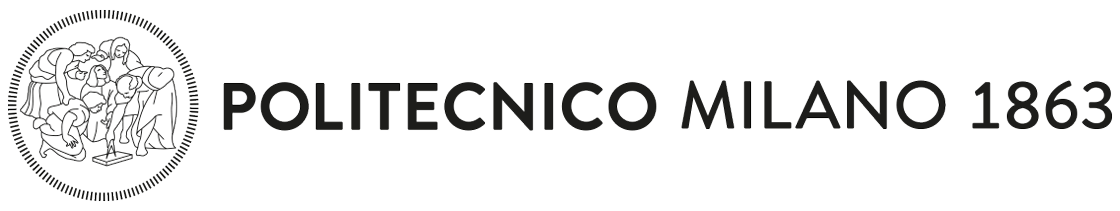
\includegraphics[width=\linewidth]{logo_politecnico.png}
  
\end{figure}
\maketitle
\tableofcontents{}

\newpage

\section{Introduction}

\subsection{Purpose}
This document provides an analysis of the CLup system in terms of assumptions, functional and non functional requirements needed to fulfill its main goals. It describes the domain in which the system will be deployed by presenting relevant scenarios and use cases and it highlights the software’s limits and constraints.\\
\smallskip\\
The document is addressed to all the stakeholders affected by the software and is meant to be used by developers in order to realize a system that meets the purpose for which it was intended.\\
\smallskip\\
The CLup system is designed to be an easy-to-use software application, meant to help both common users and store managers to face some significant difficulties due to the coronavirus emergency. In particular, the system wants to prevent people from standing in long lines outside stores and to offer them the possibility to organize in advance visits to stores. Indeed, thanks to the CLup system, people would have the chance to virtually join stores' queues and approach the stores only when their turn number is close to being called. In addiction, the system allows users to make reservations to visit stores during their preferred time slots. Given the emergency situation we are living, many stores were forced to restrict accesses in order to avoid crowds inside. For this reason, store managers as well would benefit from the CLup system, because it would give them the opportunity to keep track of the the number of people entering their stores. All these services offered by the CLup system have the purpose of minimizing risks and helping people respecting the restrictions imposed by the virus emergency.
\subsection{Scope}
\subsubsection{Description of the given problem}
As stated before, the CLup system is designed to regulate accesses to stores and manage lines in real time in order to respect restrictions imposed by the virus emergency and avoid crowds and long lines. In particular, the software is offered to both stores managers to monitor the influx of people in their buildings and to common users, allowing them to virtually “line-up” from home and book visits to the stores.\\
\smallskip\\
The main functionalities offered by CLup are the following:\\
\begin{itemize}
\item Basic service: allows stores' customers to line up from home and to approach the store only when their turn is about to arrive. In order for this lining up mechanism to work effectively, the software generates an estimation of the waiting time and alerts users when is the moment to reach the store, taking into account the time they need to get to the shop from the place they are located. The estimated time is calculated considering the number of people in the virtual line and the time spent inside the store by the costumers that are already shopping. The system is also able to optimize or increase the waiting times of users in the queue when needed. In addiction, when customers enter and exit the stores, a QR code generated by the application is scanned, allowing store managers to monitor the influx of people.
\item Advanced service: allows users to book a time-slot to visit the store. When booking, users can provide the categories of the items that they intend to purchase. The system will be able to manage visits in a finer way taking into account the store's departments that customers are going to occupy.
\end{itemize}
When customers line up or make a slot reservation they are asked to provide the expected duration of the visit. Alternatively, they can let the software itself infer it (this works only for long-term customers by analyzing the customer’s previous visits).
Be aware that the functions described above will be further detailed in the next sections of the document.
\subsubsection{World Phenomena}

\begin{figure}[H]
  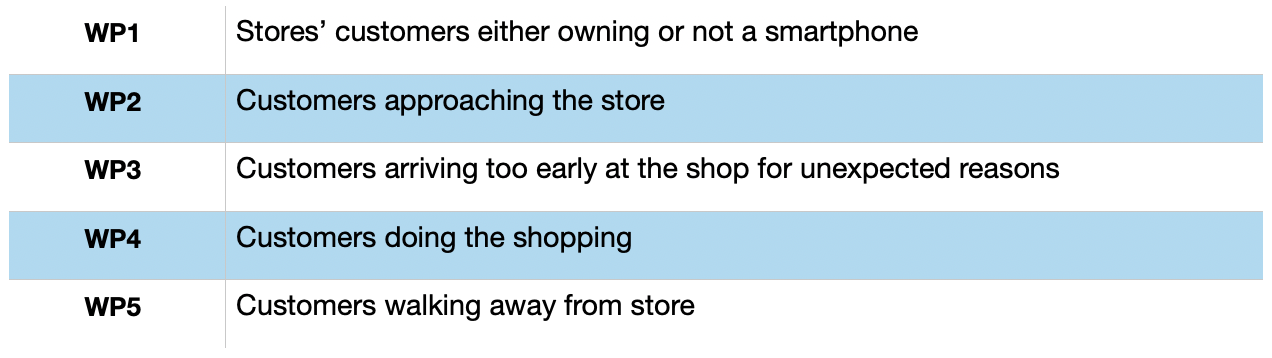
\includegraphics[width=\linewidth]{WorldPhenomena.png}
  
\end{figure}

\subsubsection{Shared Phenomena}

\begin{figure}[H]
  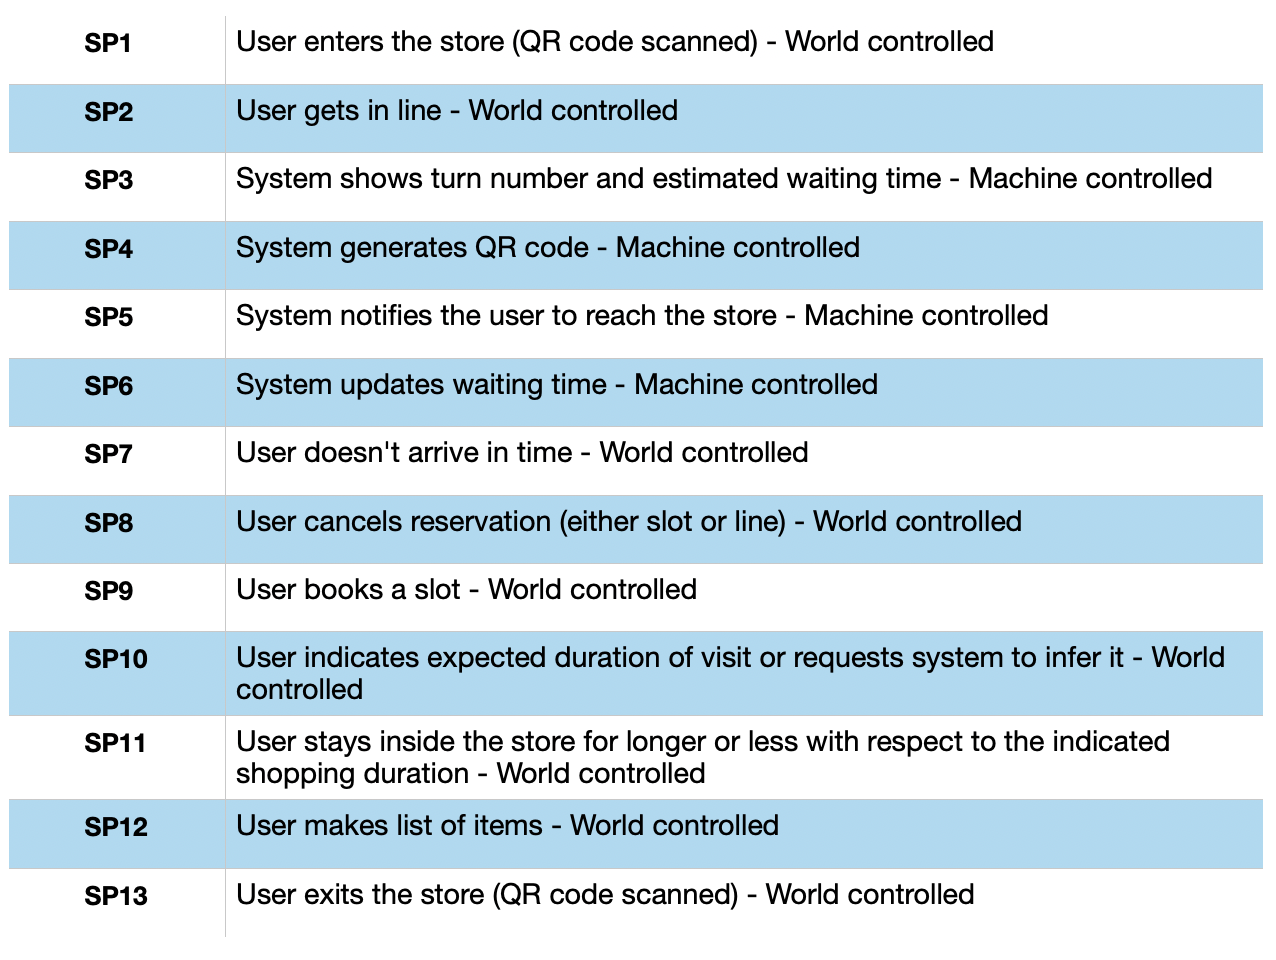
\includegraphics[width=\linewidth]{SharedPhenomena.png}
  
\end{figure}

\subsubsection{Goals}

\begin{figure}[H]
  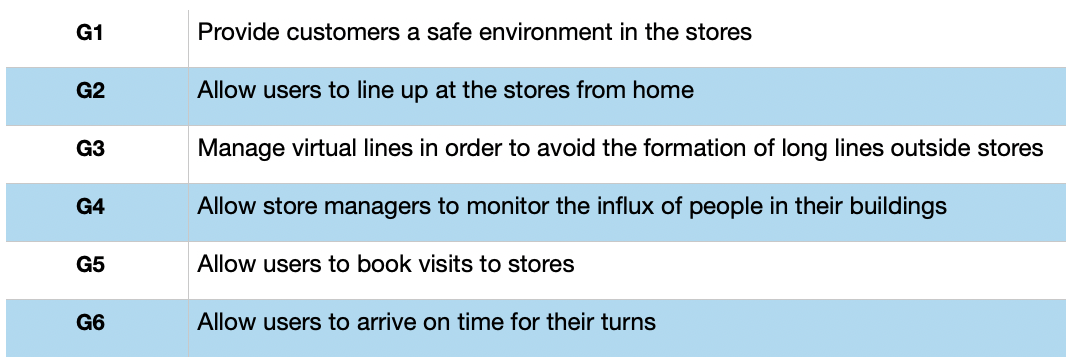
\includegraphics[width=\linewidth]{Goals.png}
  
\end{figure}

\subsection{Definitions, Acronyms, Abbreviations}
\subsubsection{Definitions}
\begin{itemize}
\item Product type: a set of similar products. Usually, items with the same product type are located in the same store's department.
\item Smart Turnstile: a turnstile equipped with a QR codes scanner.
\item Store's department: a specific section of the store, containing only a subset of all the product types
\item Store manager: the person responsible for the store and for the interactions between the store and the system. He can be helped by his employees.
\item Waiting time: an estimation of the time needed to the queue to get to a specific turn number.
\item Reservation: booked visit to a store.
\end{itemize}
\subsubsection{Acronyms}
\begin{itemize}
\item GPS: Global Positioning System
\item API: Application Programming Interface
\end{itemize}
\subsubsection{Abbreviations}
\begin{itemize}
\item WPn: n-th World Phenomena
\item SPn: n-th Shared Phenomena
\item Gn: n-th Goal
\item Dn: n-th Domain Assumption
\item Rn: n-th Functional Requirement
\end{itemize}

\subsection{Overview}
The RASD document is structured in the following 5 chapters:
\begin{itemize}
\item\textbf{Chapter 1} describes the document’s purpose and brief identification of the context in which the application is going to work given its main functionalities. It also provides lists of world phenomena, shared phenomena and goals that the system is supposed to achieve. Finally, useful specifications (definitions, acronyms, abbreviations) are included for a better understanding of the next sections of the document.
\item\textbf{Chapter 2} gives an overall description of the project. The class diagram in the Product Perspective provides a conceptual overview of the main elements of the system and the state charts describe the evolution of relevant objects. In the Product Function section, the system’s high level functionalities are further detailed and clarified. The expected type of actors that will interact with the system are listed in User Characteristics. Ultimately, chapter 2 describes the system’s constraints and the domain properties assumed to hold in the world.
\item\textbf{Chapter 3} describes the external interface requirements (user, hardware and software interfaces). Some scenarios are listed to clarify how the system works in real world situations. Both functional and non-functional requirements are described. The former are defined by several use cases and their relatives sequence diagrams, while the latter are identified though performance requirements, design constraints and software system attributes.
\item\textbf{Chapter 4} includes the Alloy model of some relevant aspects and a brief discussion of its purpose.
\item\textbf{Chapter 5} presents the effort spent by the group members while working on this project.
\item\textbf{Chapter 6} includes the reference documents.
\end{itemize}


\section{Overall Description}
\subsection{Product Perspective}
\subsubsection{Class diagram}
The class diagram below gives a high level representation of the system's domain. Classes contains only the necessary attributes to highlight the most important dynamics. \textbf{QR Code} is associated either to a \textbf{Turn Number} or to a \textbf{Reservation} and is provided with attributes required to associate the measured duration of the stay to the user. Reservation contains a list of \textbf{Product Types} and every product type is located in a specific store \textbf{Department}. A \textbf{Queue} is composed by a certain amount of \textbf{Turn numbers}. The \textbf{Distance} needs two \textbf{Positions} and can access to the time estimated by the \textbf{Maps Service API}. The \textbf{StoreManager} is able to use the webApp on the \textbf{Store's Computer},needed also to control the \textbf{Printer} and the \textbf{Display}. Moreover, \textbf{Customer} has a direct access to a list of the previous shopping times (calculated by the system using \textbf{QR Code} attributes).\newline\newline\newline\newline
\begin{figure}[H]
  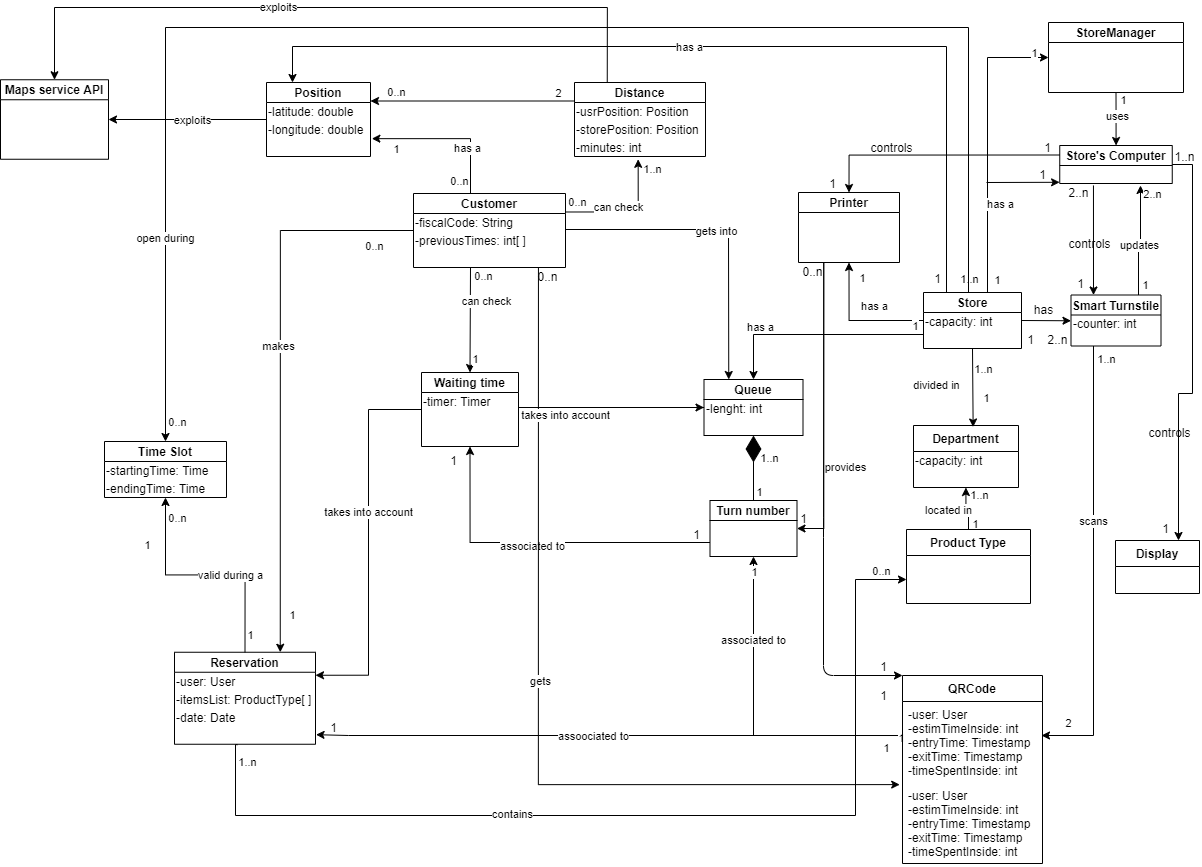
\includegraphics[width=\linewidth]{class_diagram.png}
  
\end{figure}

\newpage
\subsubsection{Statechart diagrams}

The diagrams below represent the states relative to some classes we wanted to analyse.

\begin{figure}[H]


  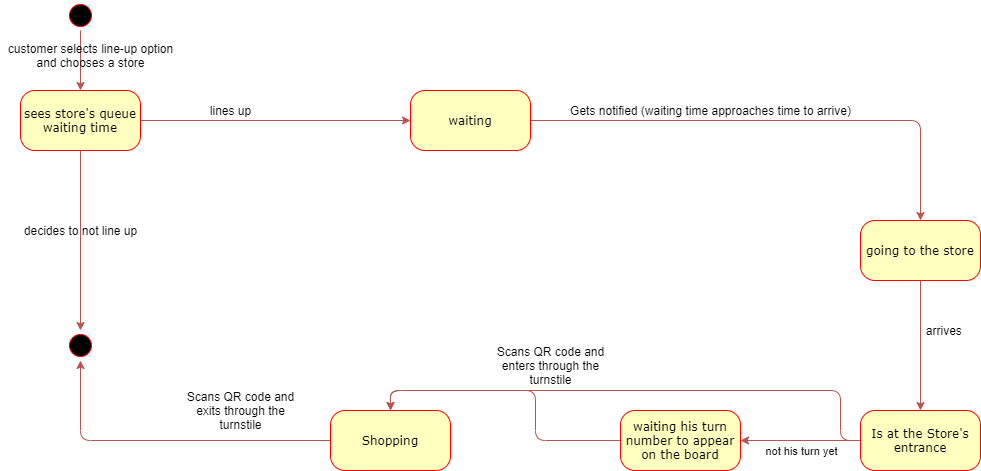
\includegraphics[width=\linewidth]{Customer_state.png}

\end{figure}

The first diagram shows the states relative to the \textbf{User} in the context of the line-up function.
\begin{figure}[H]



  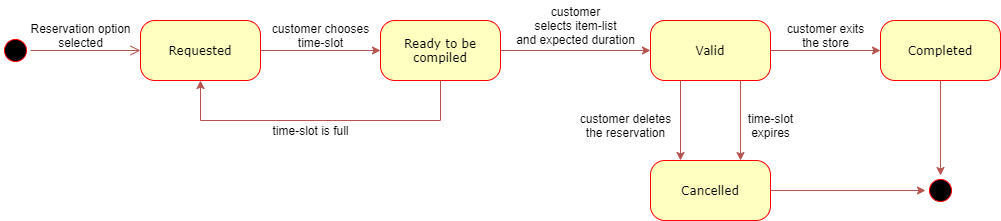
\includegraphics[width=\linewidth]{Reservation_state.png}


\end{figure}

The second diagram models the states in which a \textbf{Reservation} goes through in the context of the "booking a visit" function.\newline\newline\newline

\begin{figure}[H]

  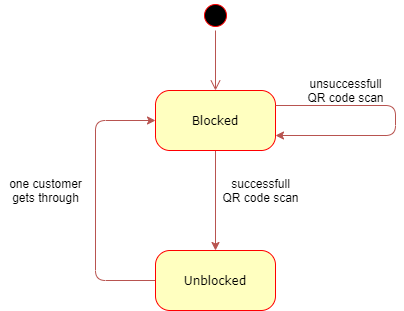
\includegraphics[width=6cm]{Turnstiles_state.png}


\end{figure}
The last one is a simple diagram, showing the functioning of the \textbf{Smart Turnstiles} positioned at the stores' entrances.

\subsection{Product Functions}
The main functions that the system will provide are listed in the following section. The identified high level requirements will be further broken down and detailed in section 3, with respect to the previously recognized goals of the system.
\subsubsection{Line up} 
As previously stated, the basic functionality allows users to virtually stand in line to enter the stores. Firstly, the user selects the store and chooses among the two available options: line up or book a visit. Whenever the choice is to line up, the system will show to the user the estimated waiting time to enter. At that point, if the user decides to actually get in the line, he/she will be asked to provide the expected duration of the visit and finally, he/she will receive the turn number and the QR code that has to be scanned when entering to the store. The user will be asked wether he/she will reach the store on foot or by car, so that the system will be able to calculate the user's expected time needed to reach the store (exploiting a Maps Service API). This time will be shown to the user while he/she is waiting, together with the waiting time (constantly updating). The user will be notified by the system when the time he/she needs to get to the store equals the time left for the user to enter. Once arrived to the store, the user might need to wait few minutes until his/her number appears on the queue board. Finally, the smart turnstile will scan the QR code and unlock, letting the user enter the store and start shopping.
\subsubsection{Book a visit} 
As mentioned before, after choosing the store, the user also has the option to book a visit. He/she will select the preferred time slot and make a reservation whenever the slot is not already full. A QR code is generated and the user can access to the store at any moment of the time slot, as long as he/she exits before the end of it. When making the reservation, the user is asked to provide the expected duration of the visit and to select the categories of items that he/she intends to purchase. This last information is used by the system to understand which store’s department the customers are going to occupy in order to manage entrances in a finer way. In particular the system can either let more people in if the distribution is homogeneous inside the store or slow down the influx of people if customers are gathered in certain departments.
\subsubsection{Manage lines} 
The CLup system has to manage the lining up mechanism effectively. First of all, the waiting time assigned to customers that get in line, can change depending on several events. In particular, whenever a customer either gets out of the line or cancels a slot reservation, the system is able to decrease the waiting times of the users currently in line and optimize the influx of people. The waiting time can also decrease in the event that someone does not show up when his/her turn is arrived (there will be a fixed maximum delay tolerated by the system). Each user (for both the basic and advanced functionality) is asked to provide the expected amount of time they intend to spend inside the store, alternatively, users can choose to let the system infer that time (only if the system has enough data). Indeed, for each user, the system will collect and store informations about the duration of his/her visits and estimate an average. As a consequence, whenever a user’s visit lasts longer or less than the estimated time, the waiting time of the users in line can be optimized (increased or decreased). Ultimately, the system is also able to handle people who do not have access to the required technology. The store manager (or one of his employees) will print a number and a QR code for those who have to physically get in line and the system will take them into account when scheduling the next entrances (they will be assigned a fixed time of stay in the shop).
\subsubsection{Keep track of accesses} 
The CLup system is also meant to be used by store managers to keep track of entrances in their buildings. This is possible thanks to the smart turnstiles that scan the QR codes. The system check the validity of the QR codes (not expired or false) and allow the turnstiles to unlock to let people in or out. Consequentially, a customer counter is updated  so that stores managers can check whether their store’s capacity is respected.
\subsection{User Characteristics}
The application is supposed to be used by the following actors:
\begin{enumerate}
\item\textbf{Registered user}: someone who downloaded the application on his/her device, registers to CLup and uses its services.\medskip\\
Depending on the service used, the following distinction can be done: 
\begin{itemize}
\item Line up: the user is someone that wants to enter the store as soon as possible and might not live too far from it. Indeed, he/she prefers to line up and is ready to move even if the waiting time is shortened.
\item Book a visit: the user is someone who plans on visiting the store in advance and at a fixed time.
\end{itemize}
\item\textbf{Unregistered user}: someone who do not have access to the required technology and therefore is not registered to CLup services. The only way in which he/she interacts with the system is by physically retrieving a turn number and a QR code from the ticket dispenser located at the store. The system will take into account this actor when scheduling the next entrances
\item\textbf{Store manager}: someone who is responsible for managing a store and registers to CLup to monitor the influx of people in his/her building.
\end{enumerate}
\subsection{Assumptions and Dependancies}
\subsubsection{Domain assumptions}
\begin{figure}[H]
  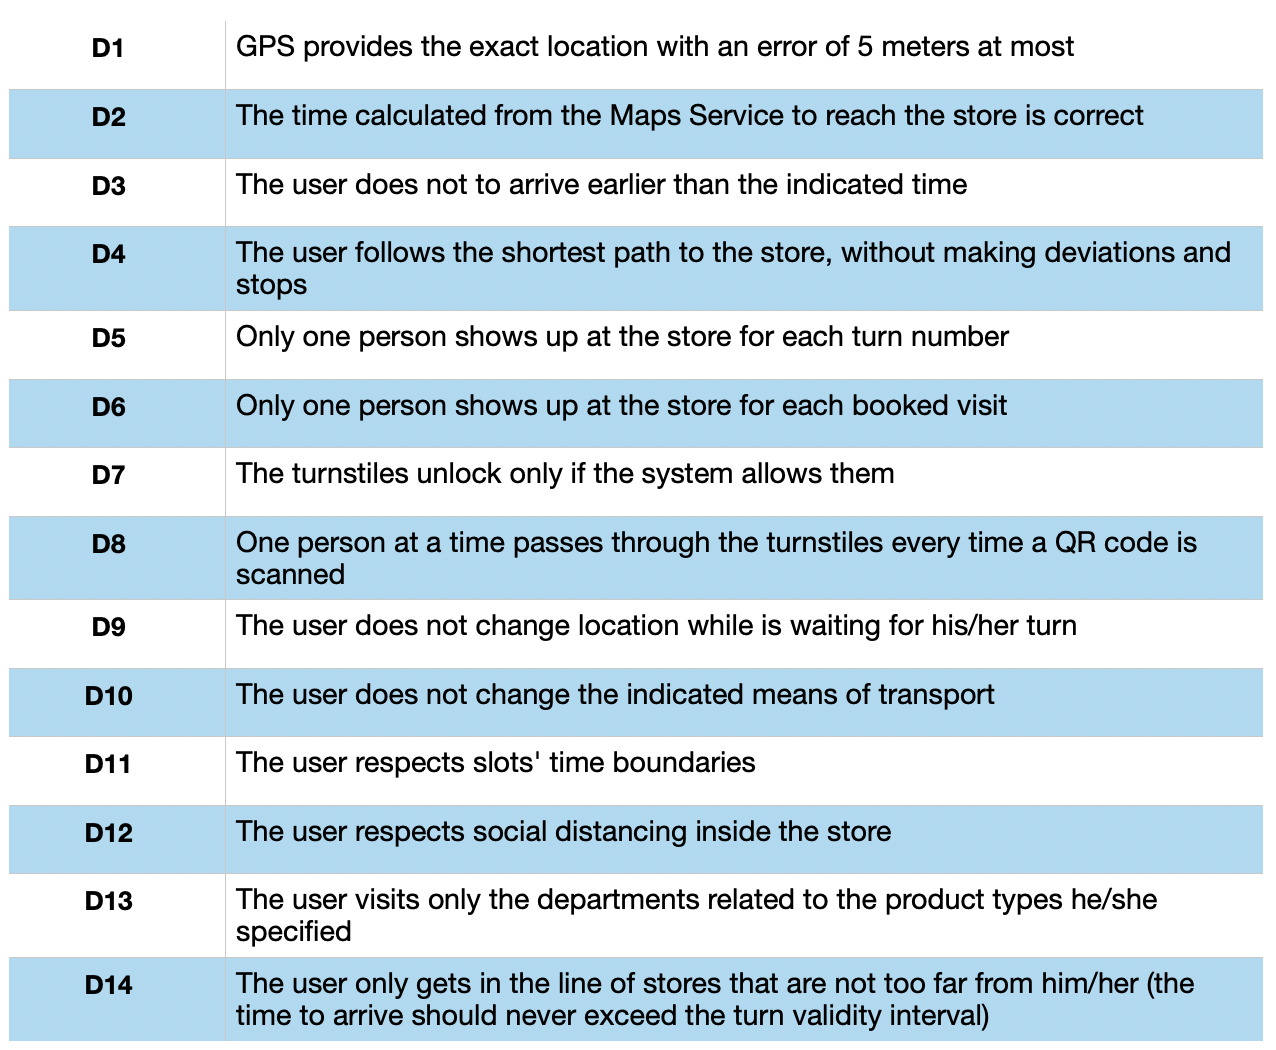
\includegraphics[width=\linewidth]{Domains.png}
  
\end{figure}

\section{Specific Requirements}
\subsection{External Interface Requirements}
\subsubsection{User Interfaces}
The following mockups give an idea of how the application looks like on the user’s smartphone. They show some screenshots of the most relevant interactions between the system and the registered users.

\begin{figure}[H]
\begin{minipage}[b]{0.4\textwidth}
\centering
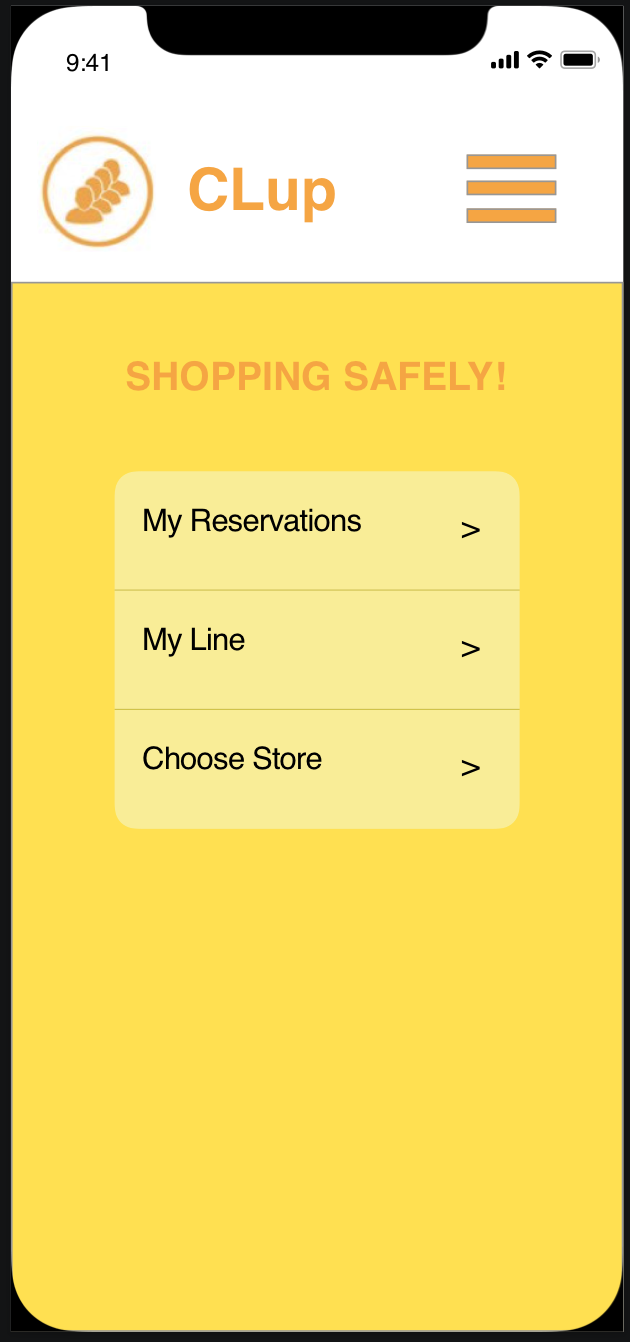
\includegraphics[width=\textwidth]{home.png}
\caption{Home}
\end{minipage}
\hfill
\begin{minipage}[b]{0.4\textwidth}
\centering
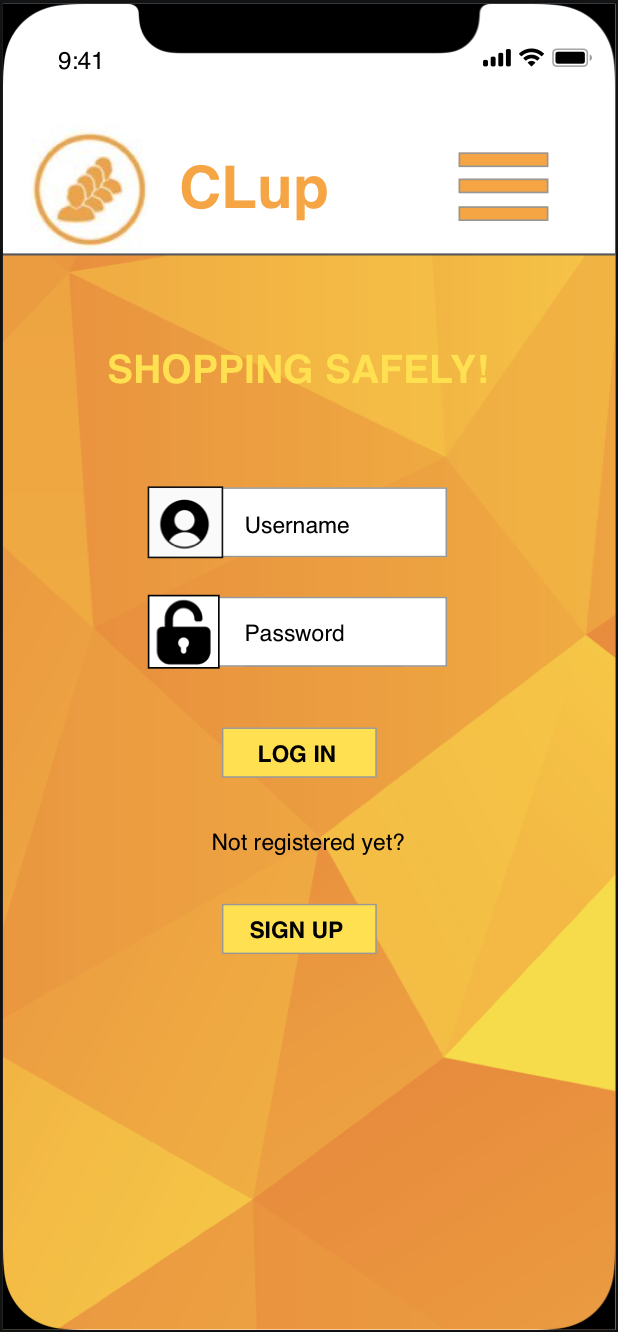
\includegraphics[width=\textwidth]{login.png}
\caption{Login}
\end{minipage}
\end{figure}

\begin{figure}[H]
\begin{minipage}[b]{0.4\textwidth}
\centering
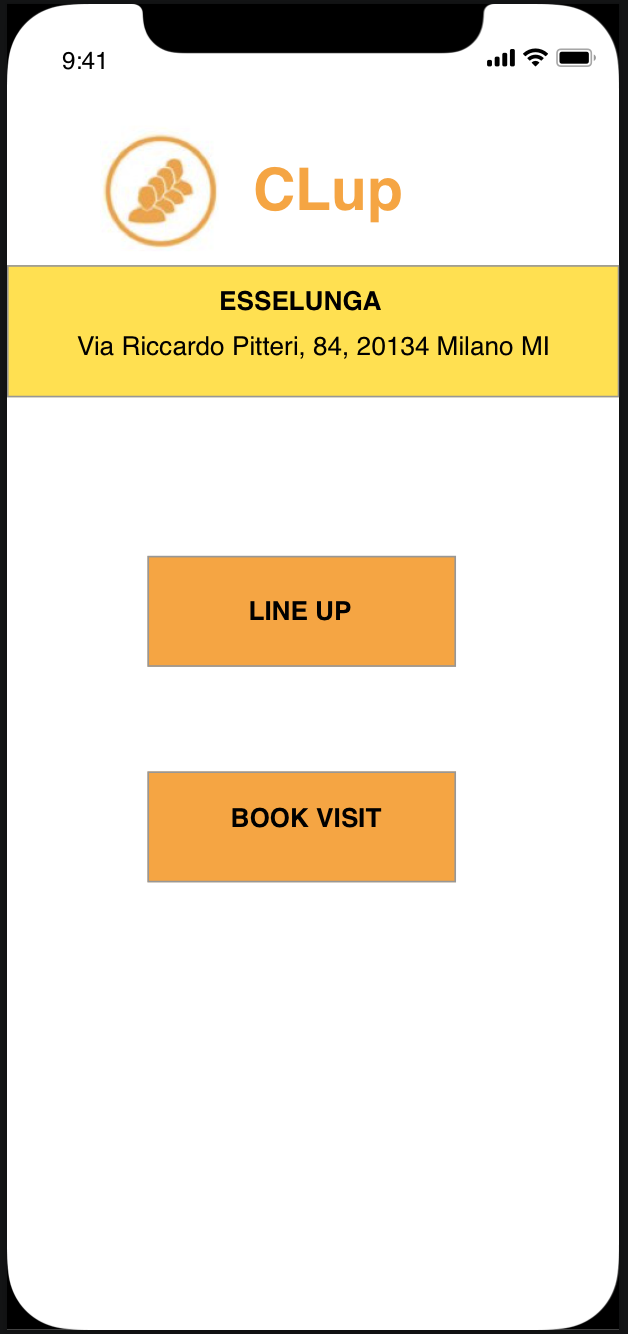
\includegraphics[width=\textwidth]{FunctionalitySelection.png}
\caption{Functionality selection}
\end{minipage}
\hfill
\begin{minipage}[b]{0.4\textwidth}
\centering
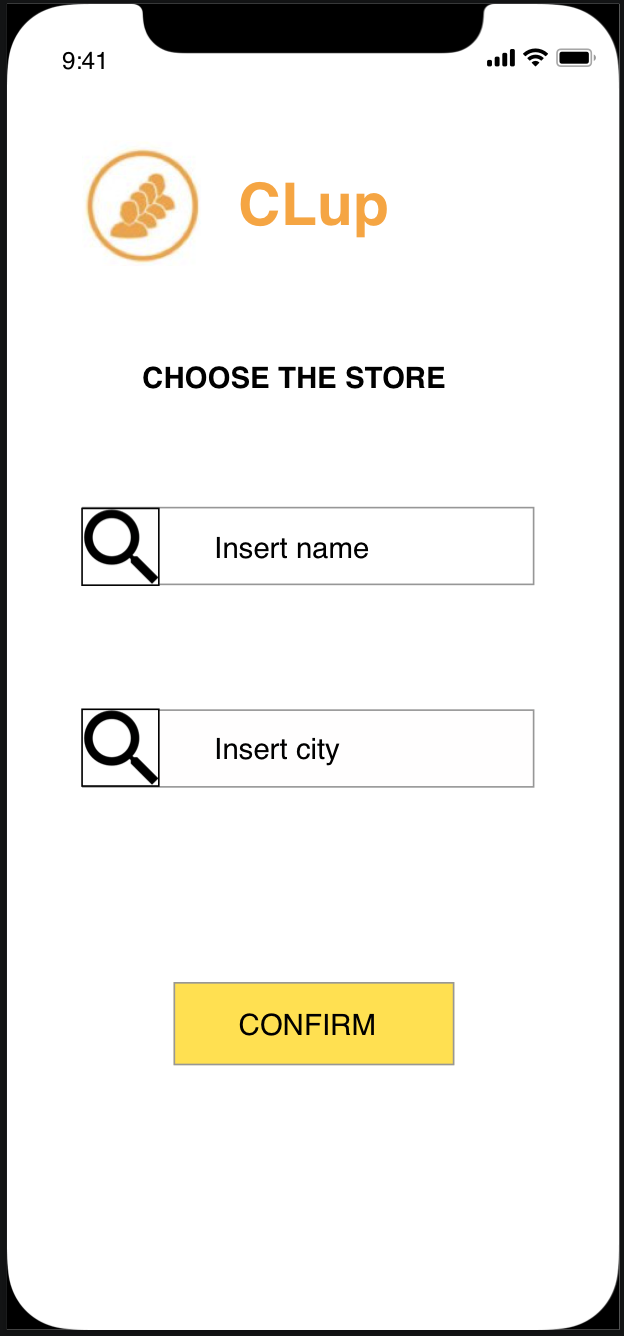
\includegraphics[width=\textwidth]{ChooseStore.png}
\caption{Store's name and city selection}
\end{minipage}
\end{figure}

\begin{figure}[H]
\begin{minipage}[b]{0.4\textwidth}
\centering
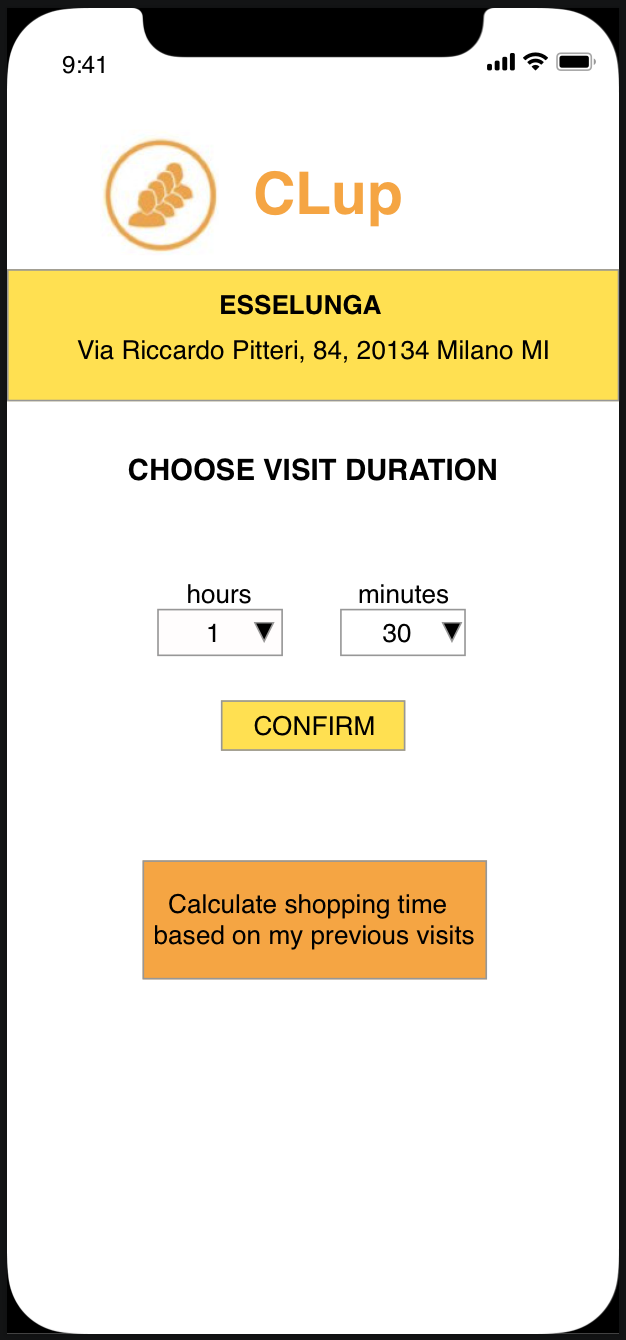
\includegraphics[width=\textwidth]{VisitDuration.png}
\caption{Shopping time selection}
\end{minipage}
\hfill
\begin{minipage}[b]{0.4\textwidth}
\centering
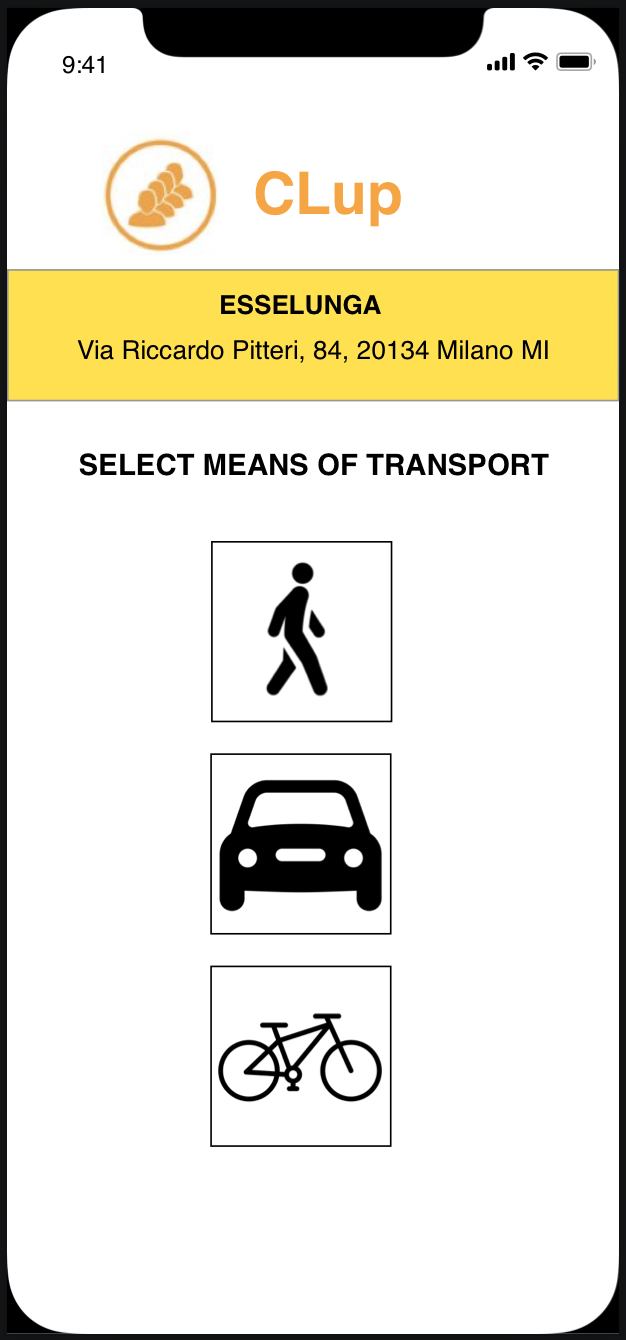
\includegraphics[width=\textwidth]{MeansofTransport.png}
\caption{Means of transport selection}
\end{minipage}
\end{figure}

\begin{figure}[H]
\begin{minipage}[b]{0.4\textwidth}
\centering
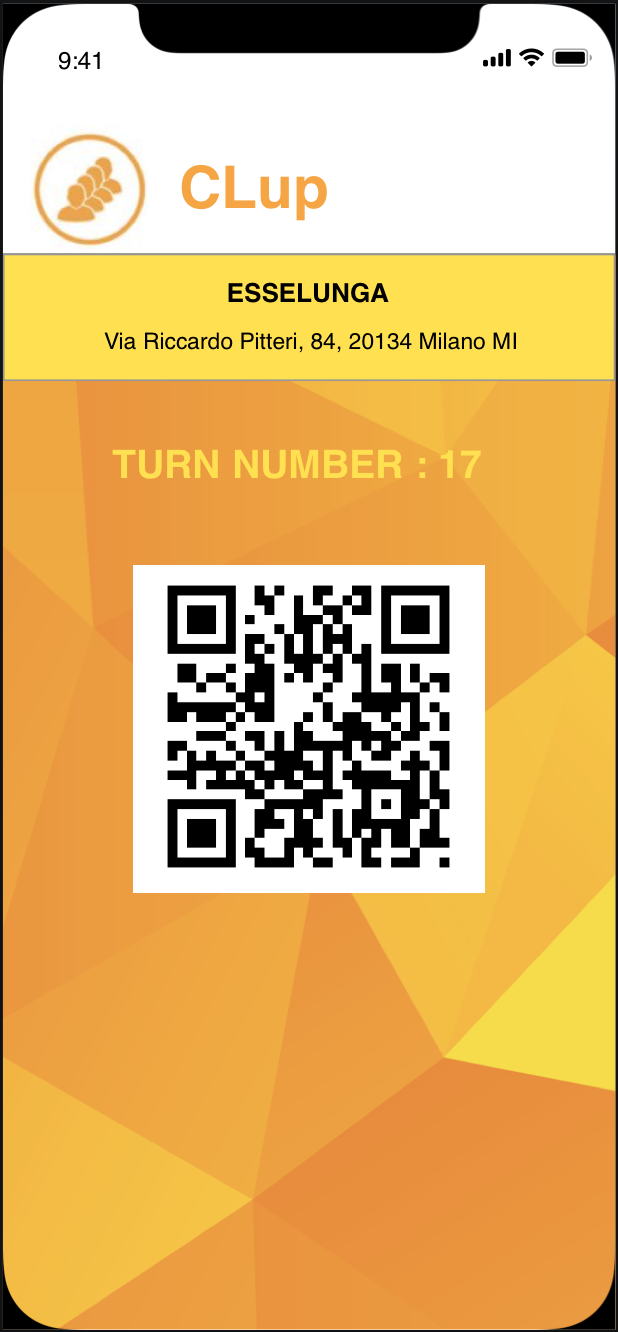
\includegraphics[width=\textwidth]{QRcode.png}
\caption{QR code}
\end{minipage}
\hfill
\begin{minipage}[b]{0.4\textwidth}
\centering
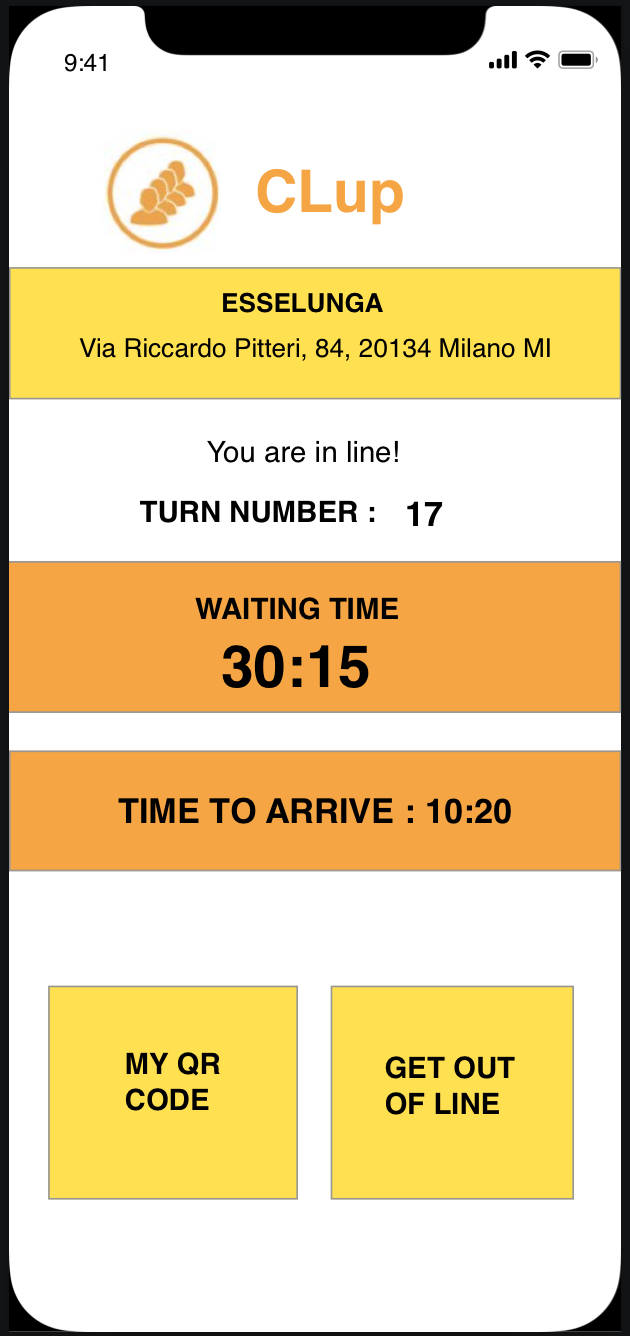
\includegraphics[width=\textwidth]{Waiting.png}
\caption{Line informations}
\end{minipage}
\end{figure}

\begin{figure}[H]
\begin{minipage}[b]{0.4\textwidth}
\centering
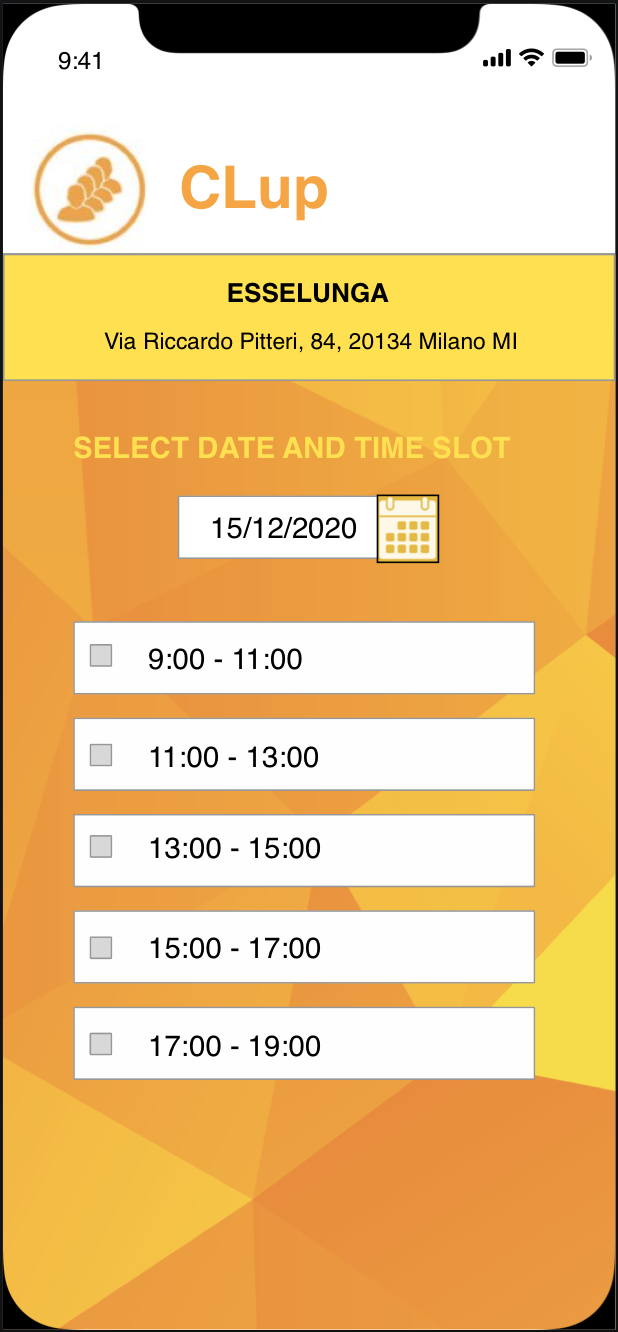
\includegraphics[width=\textwidth]{Timeslot.png}
\caption{Timeslot and date selection}
\end{minipage}
\hfill
\begin{minipage}[b]{0.4\textwidth}
\centering
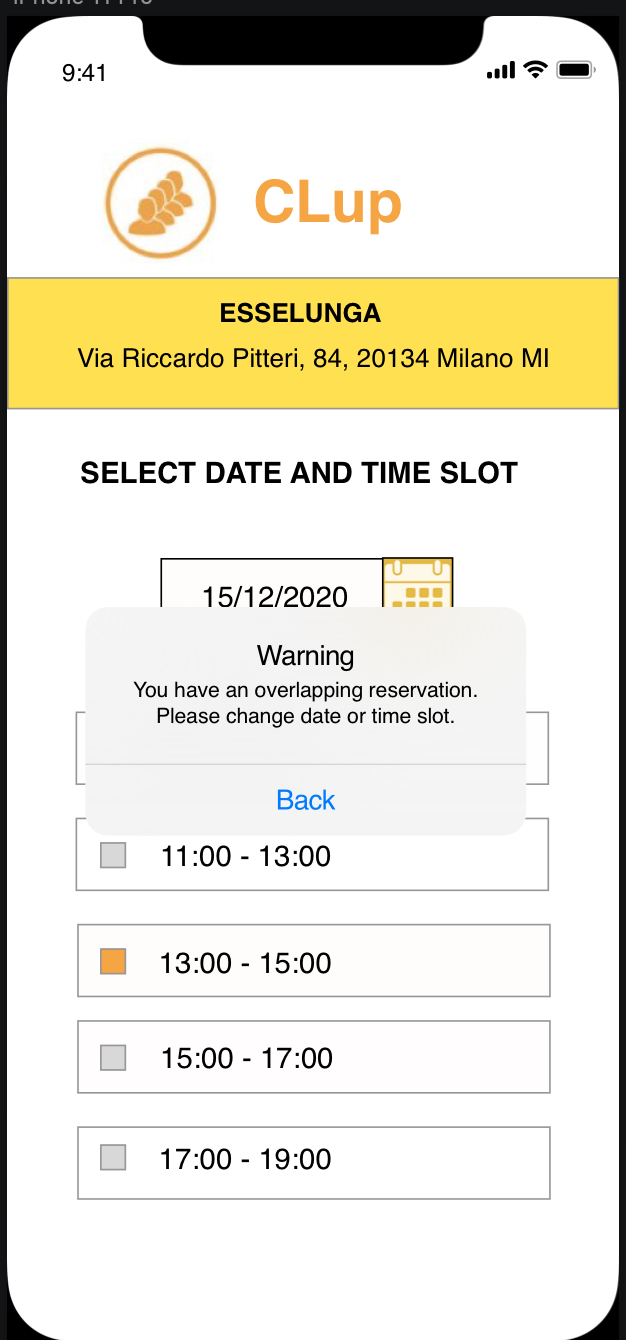
\includegraphics[width=\textwidth]{Warning.png}
\caption{Overlapping reservations warning}
\end{minipage}
\end{figure}

\begin{figure}[H]
  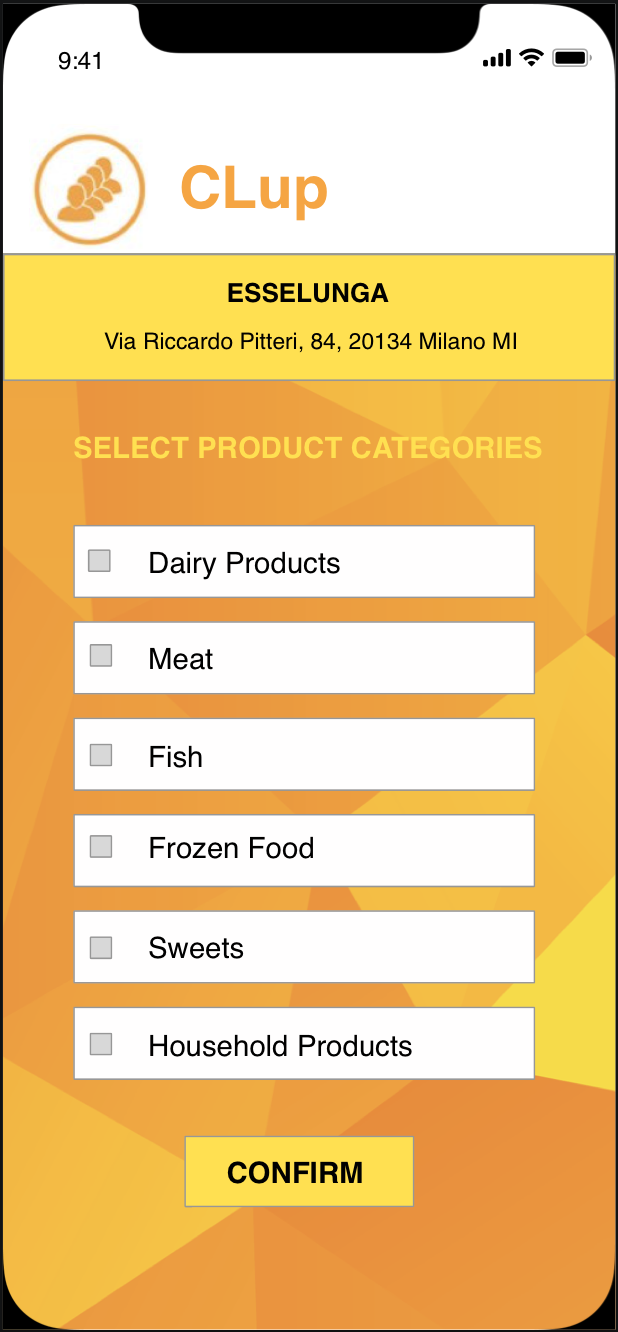
\includegraphics[width=0.4\linewidth]{ProductCategories.png}
  \centering
  \caption{Product categories selection} 
\end{figure}

\begin{figure}[H]
  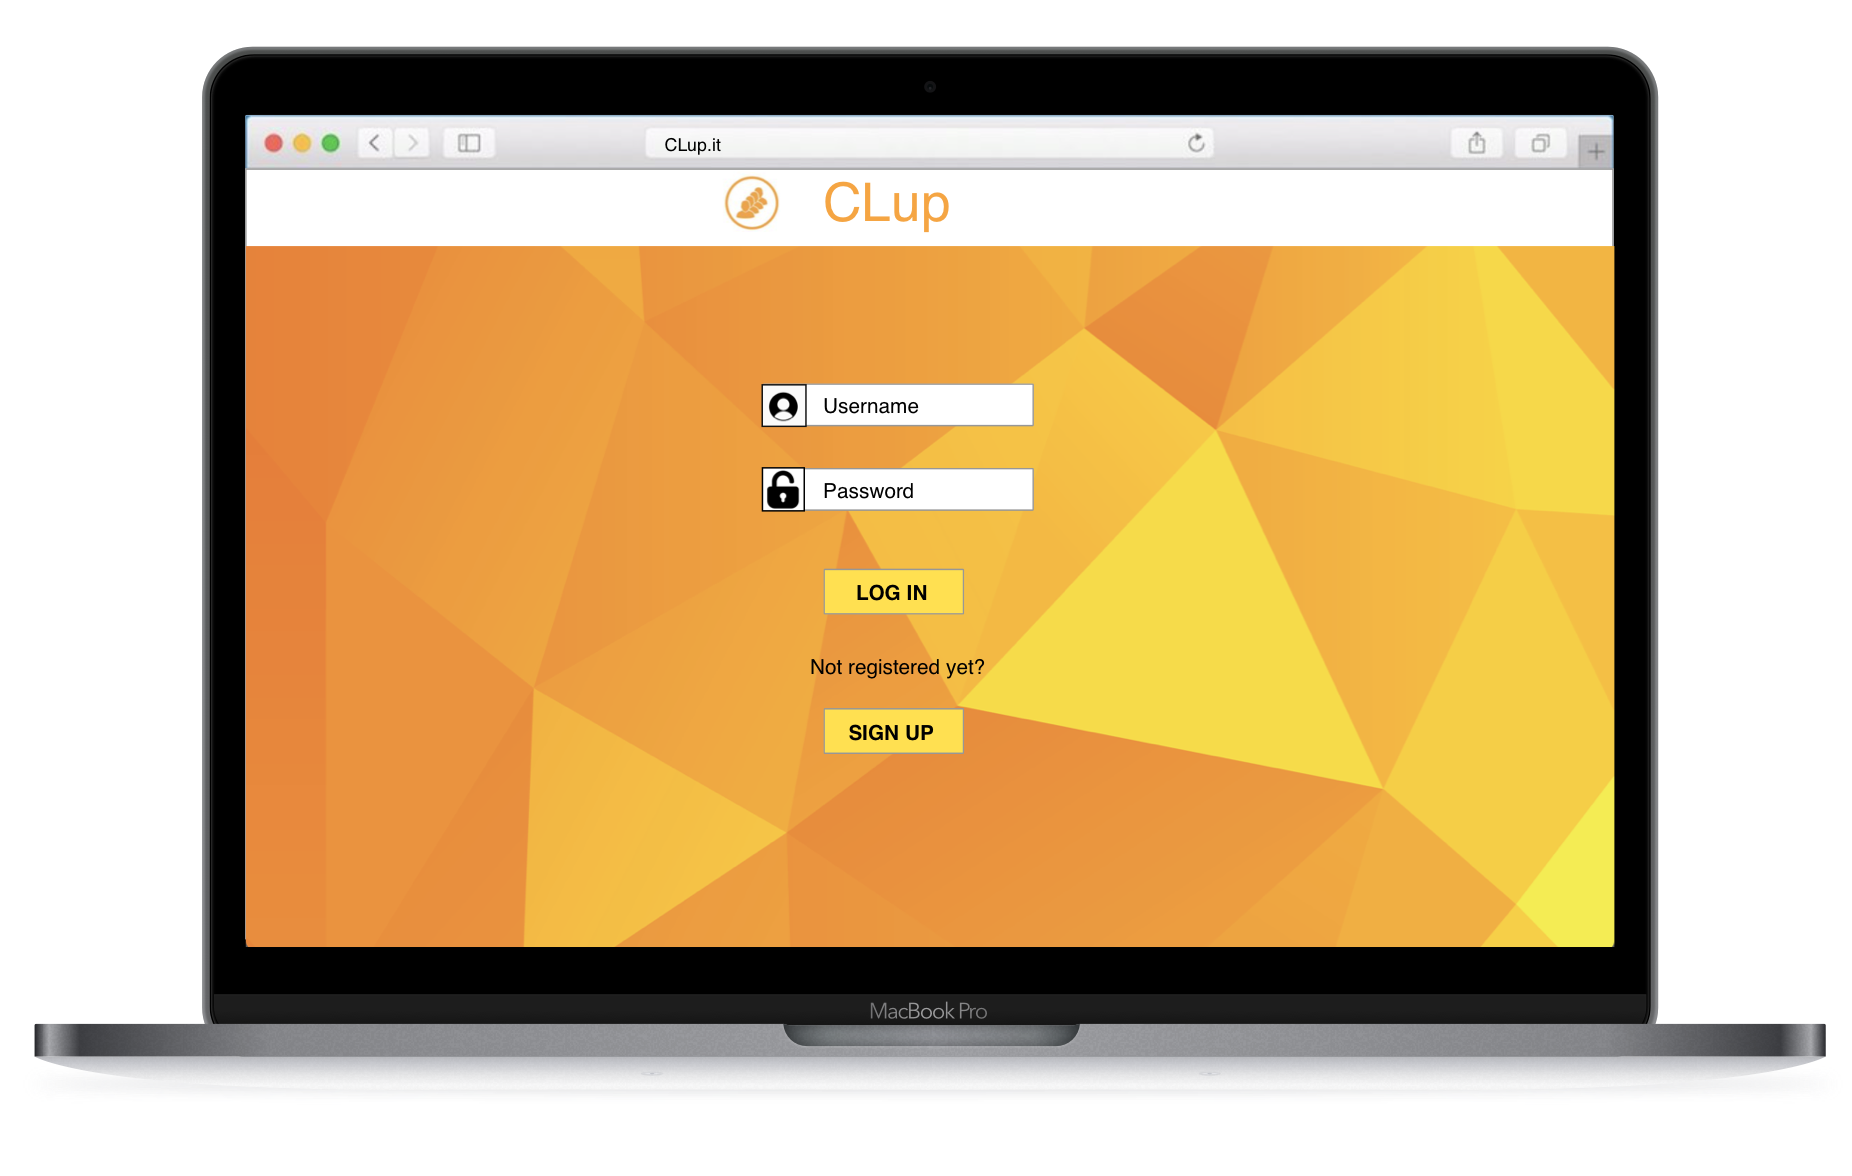
\includegraphics[width=\linewidth]{WebAppLogin.png}
  \centering
  \caption{WebApp Login} 
\end{figure}

\begin{figure}[H]
  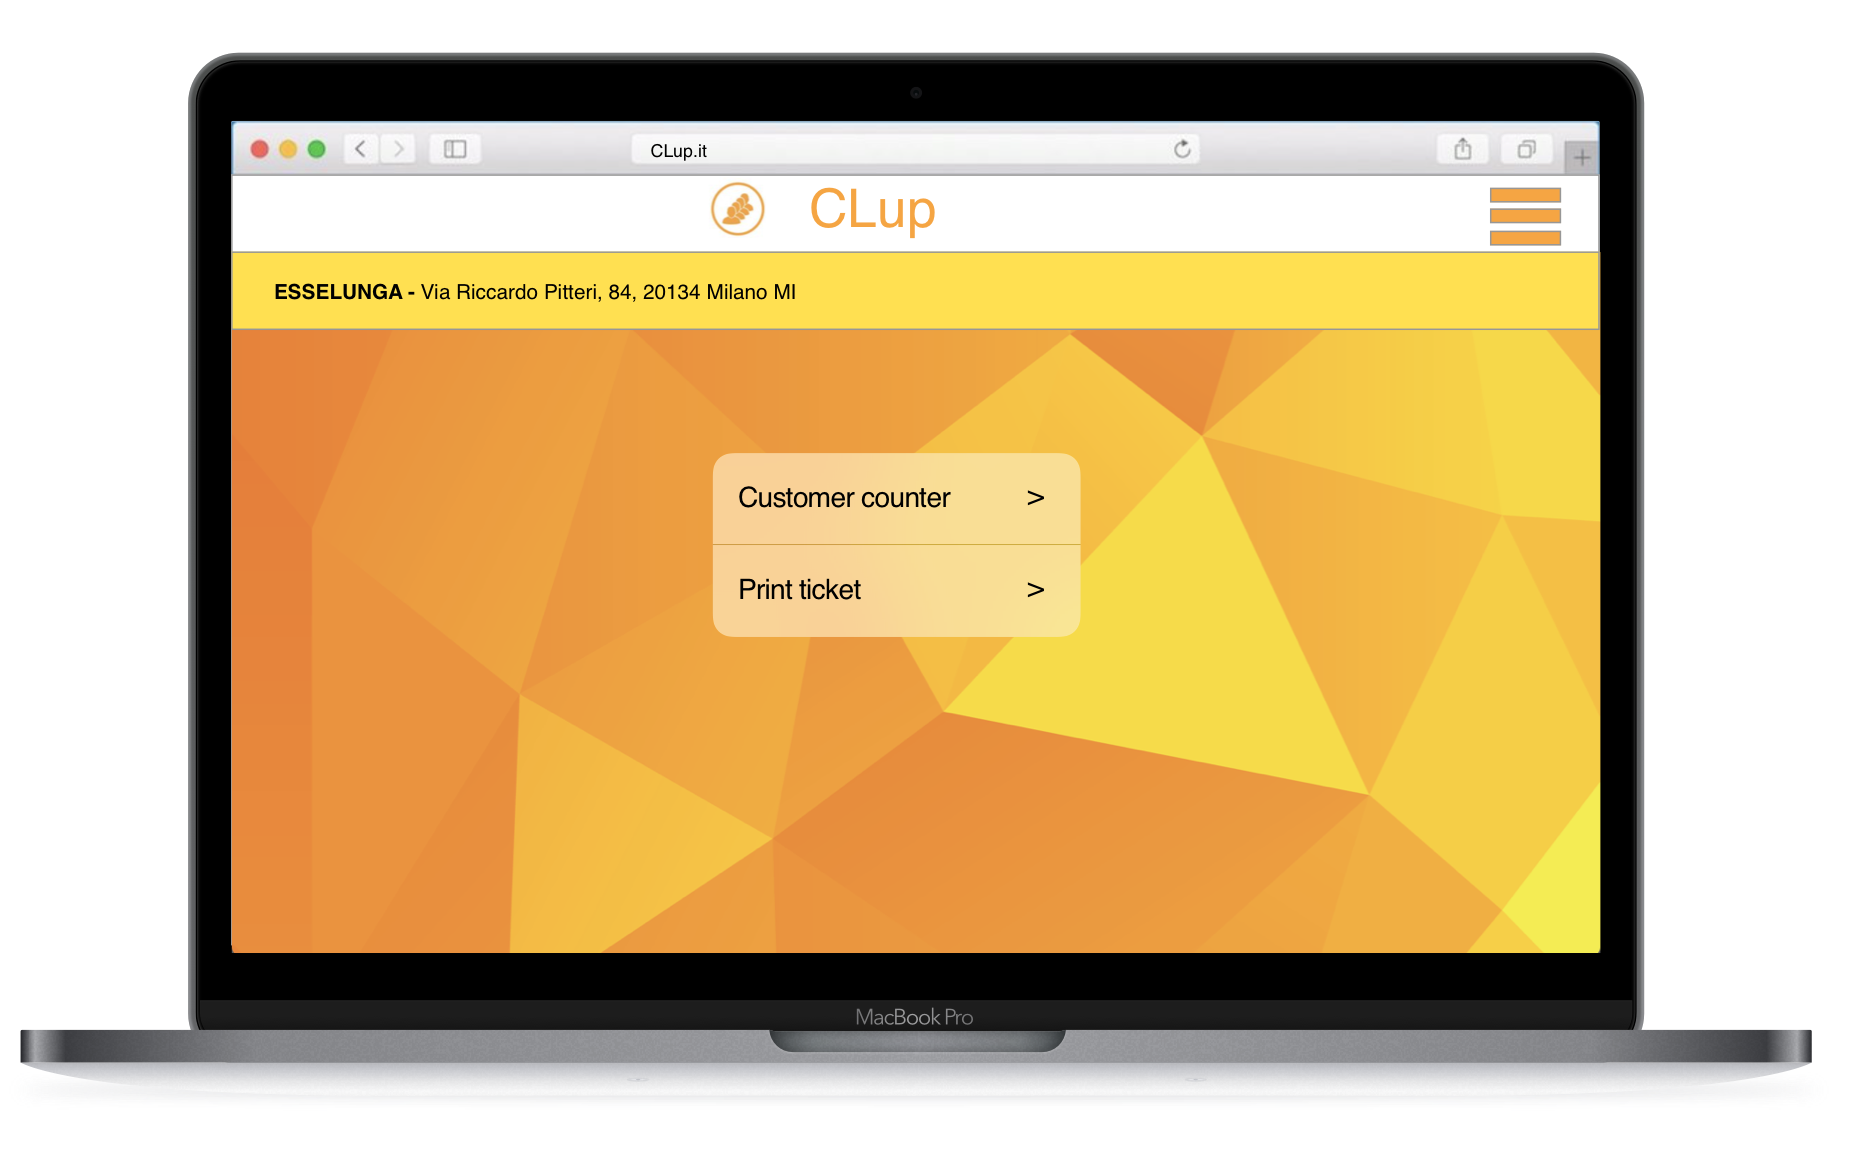
\includegraphics[width=\linewidth]{WebAppHome.png}
  \centering
  \caption{WebApp Home} 
\end{figure}

\begin{figure}[H]
  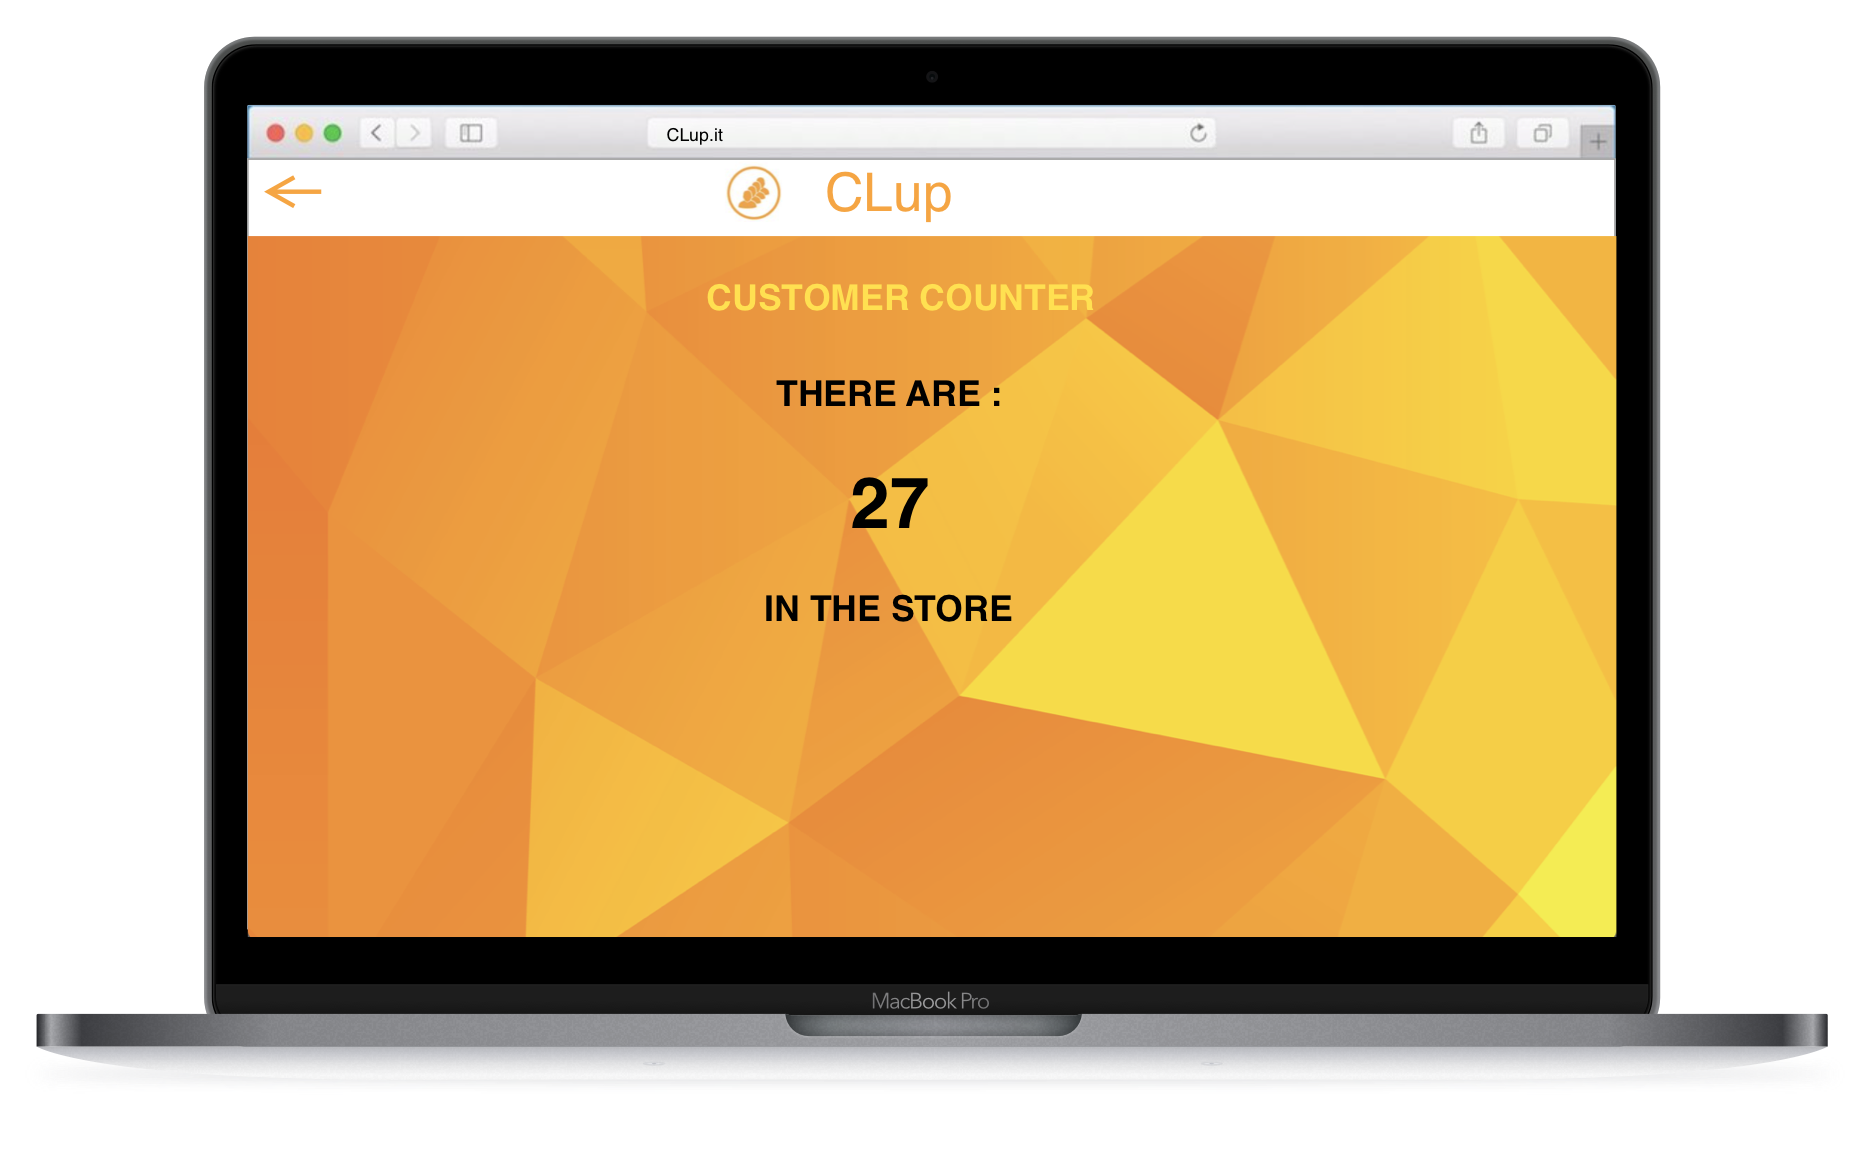
\includegraphics[width=\linewidth]{CustomerCounter.png}
  \centering
  \caption{Customer counter} 
\end{figure}

\begin{figure}[H]
  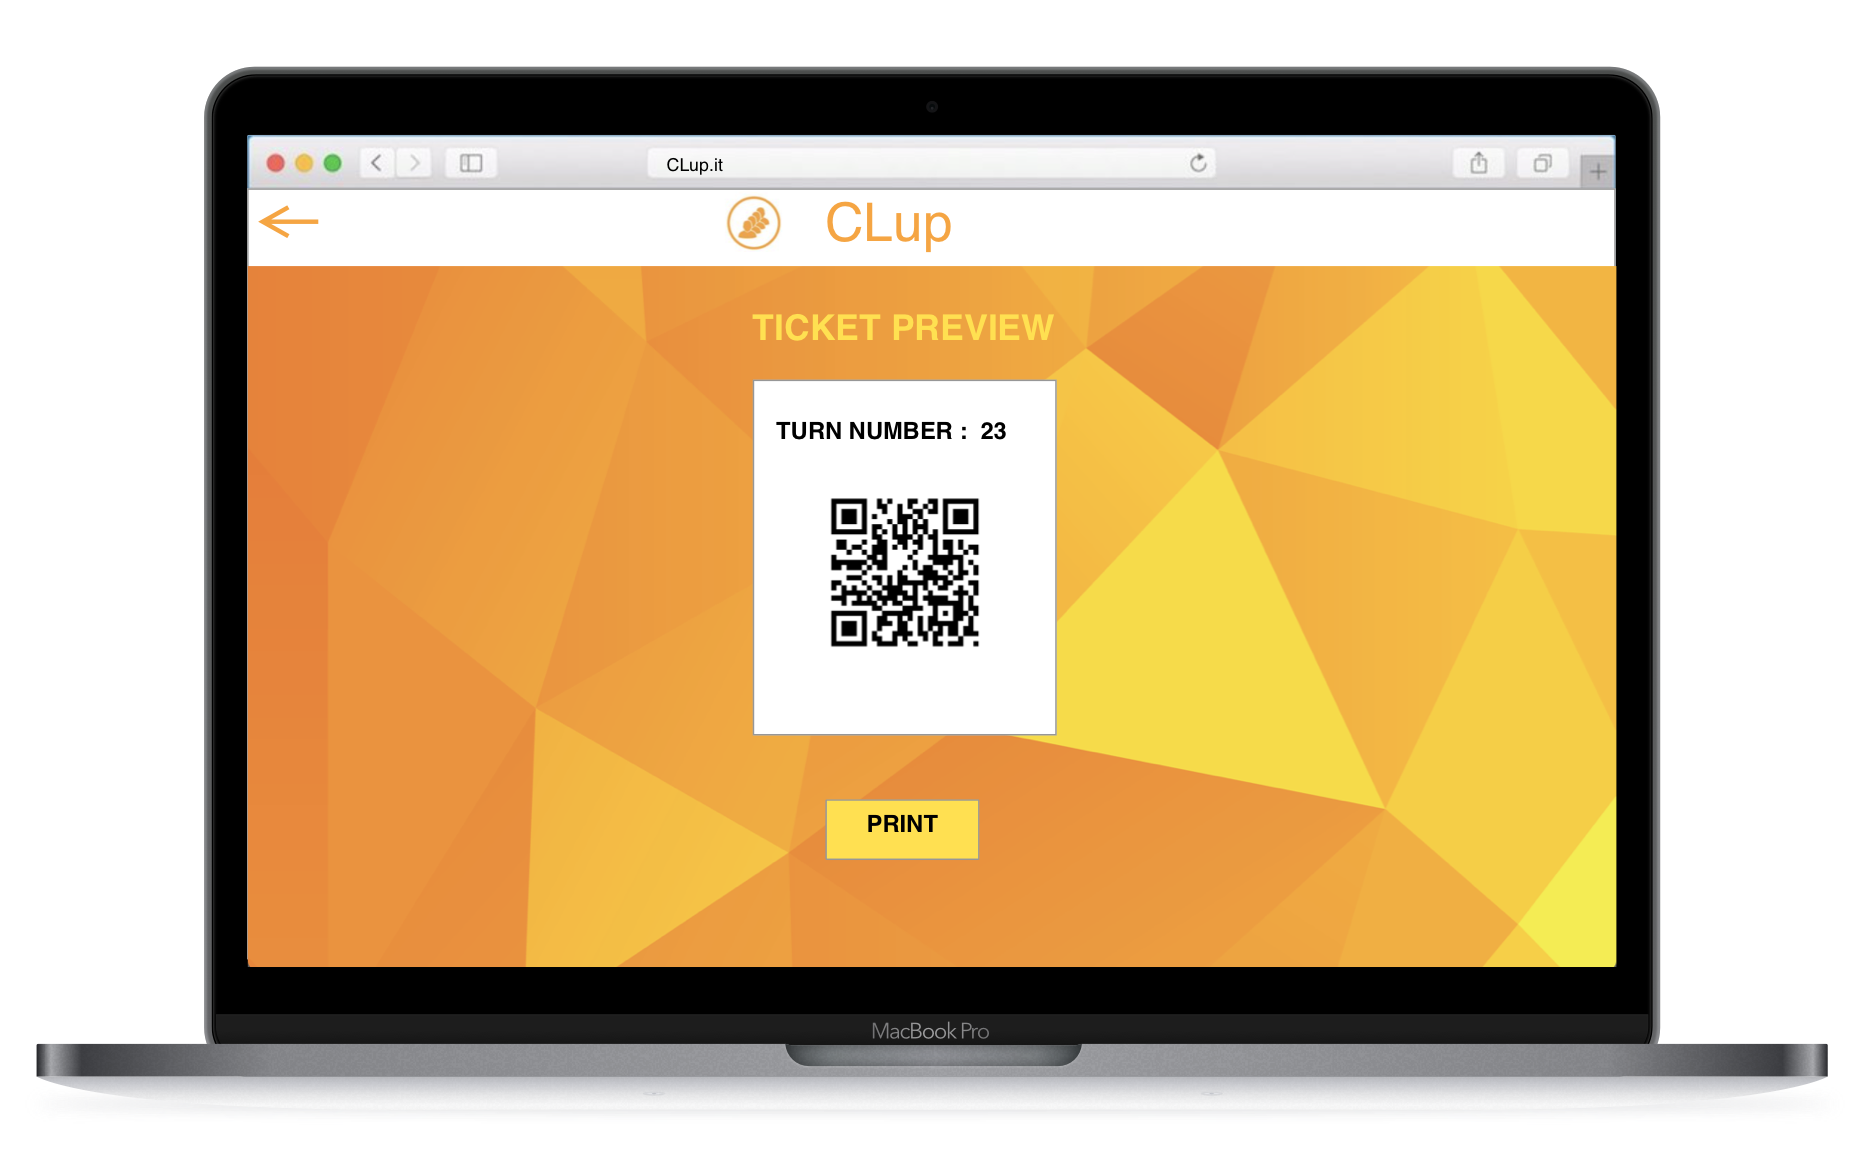
\includegraphics[width=\linewidth]{TicketPreview.png}
  \centering
  \caption{Ticket preview} 
\end{figure}





\subsubsection{Hardware Interfaces}
The required hardware interfaces are listed below:
\begin{itemize}
\item Users must own a smartphone in order to download CLup’s application and use its services.
\item At least one computer and a printer are required in the stores, so that the store manager (or one of his employees) is able to access CLup’s WebApp, check the customer counter and print physical tickets.
\item Turnstiles able to scan QR codes must be placed at the entrances of stores in order to control the influx of people.
\item Stores must be equipped with a display that shows and communicates (by generating sound) the current turn number.
\end{itemize}
\subsubsection{Software Interfaces}
The external interfaces required by the system are listed below:
\begin{itemize}
\item Position: the system uses a Maps Service API to retrieve the position of the user when he/she gets into a line in order to calculate his/her distance from the store and to show to the user the estimated time needed to reach the store.
\item Turnstile: the system needs to communicate with the turnstiles' software in order to receive the informations related to the scanned QR codes and to the entrances/exits timestamps. This communication occurs between the store's computer and the turnstiles' integrated controller over LAN.
\end{itemize}
\subsection{Functional Requirements}
\subsubsection{List of Requirements}

\begin{figure}[H]
  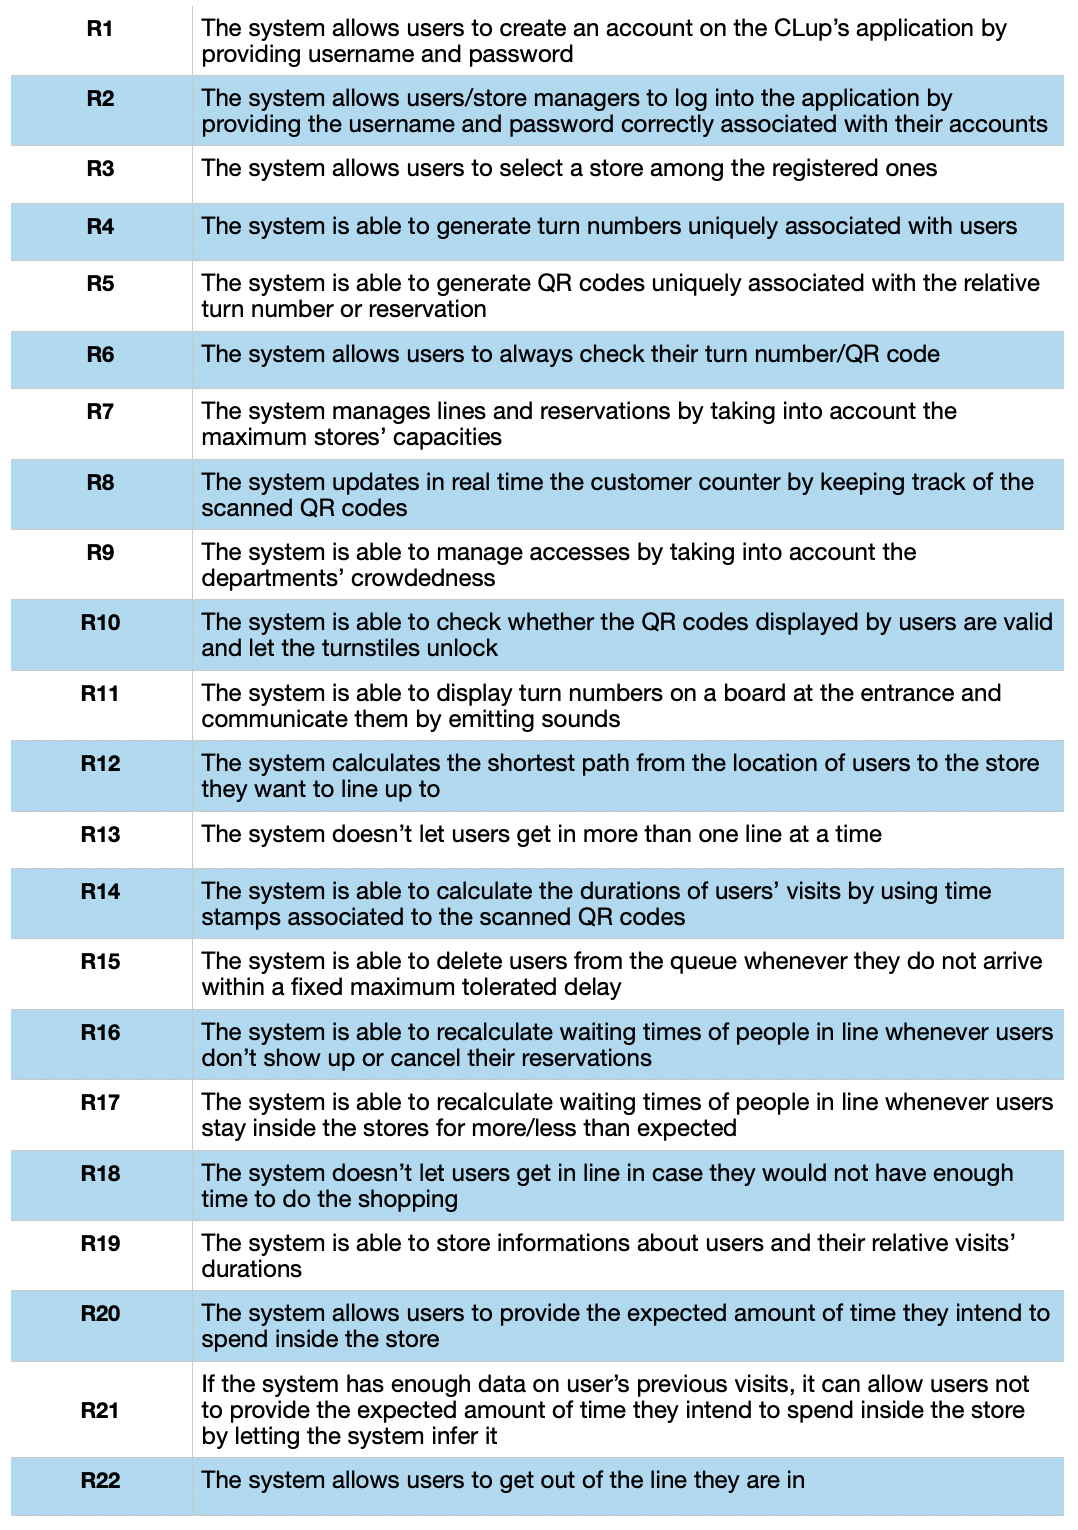
\includegraphics[width=\linewidth]{Requirements1.png}
  
\end{figure}
\begin{figure}[H]
  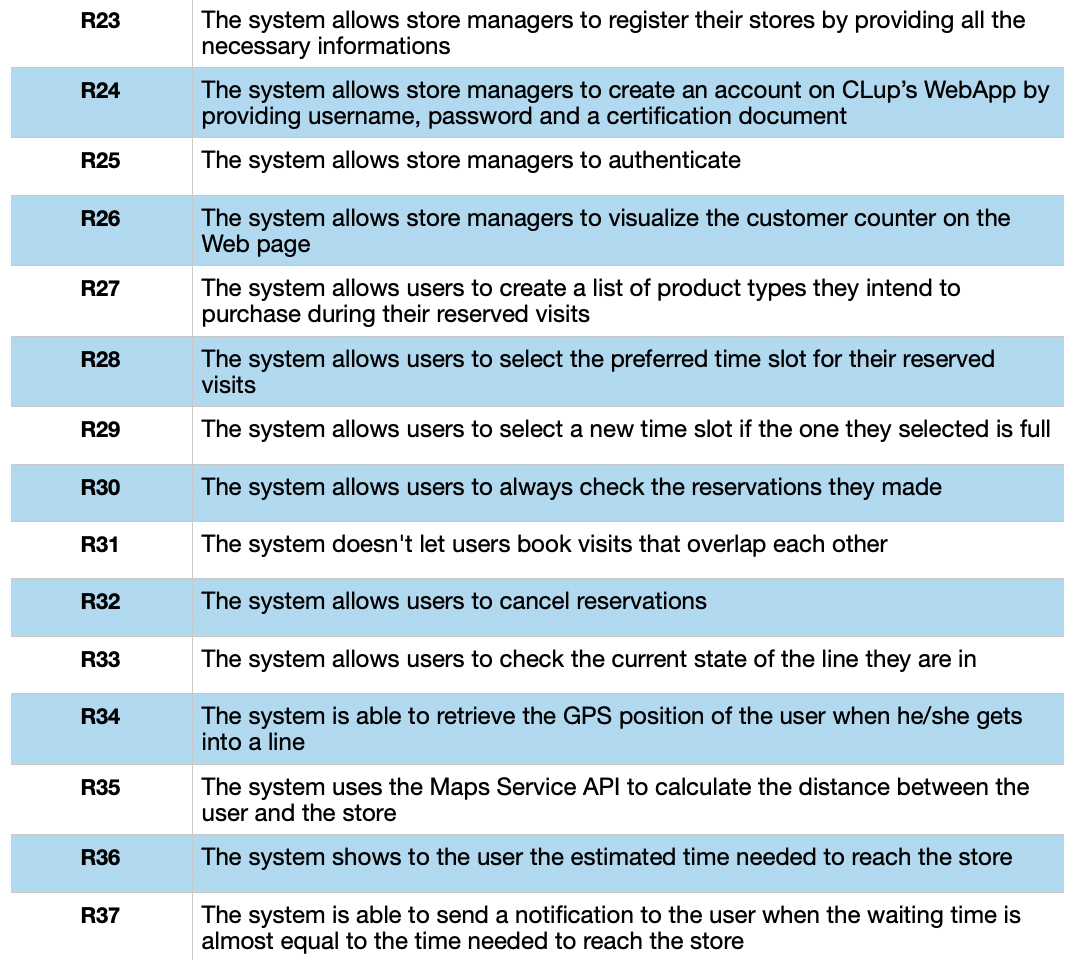
\includegraphics[width=\linewidth]{Requirements2.png}
  
\end{figure}

\subsubsection{Mapping}
In this section, each Goal is associated with the Requirements that ensure the satisfaction of it, in the context of the Domain Assumptions.

\begin{figure}[H]
  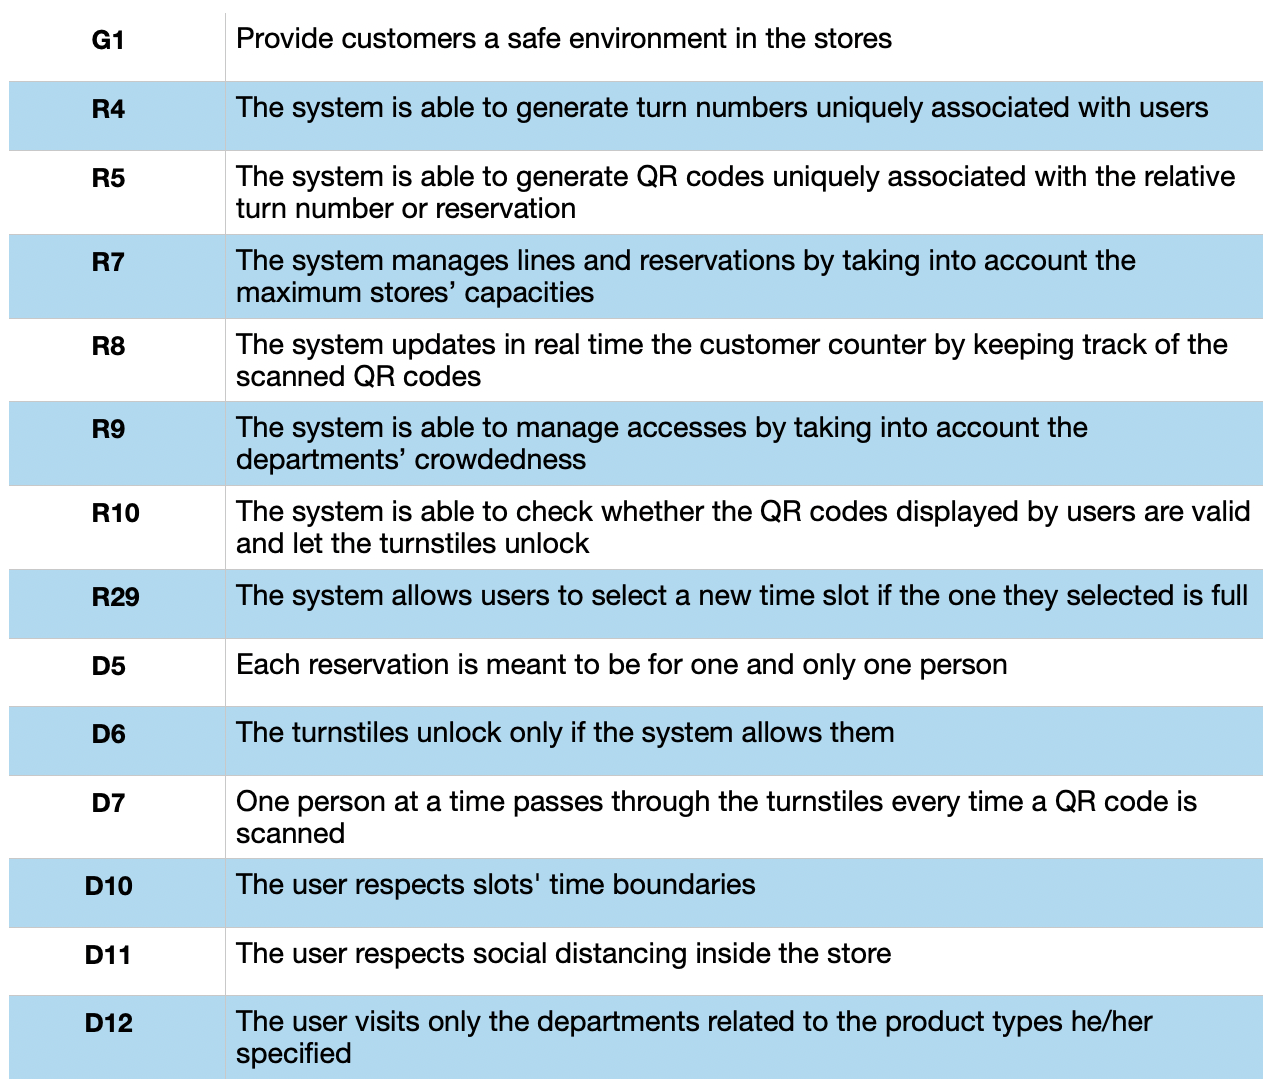
\includegraphics[width=\linewidth]{Mapping1.png}
  
\end{figure}

\begin{figure}[H]
  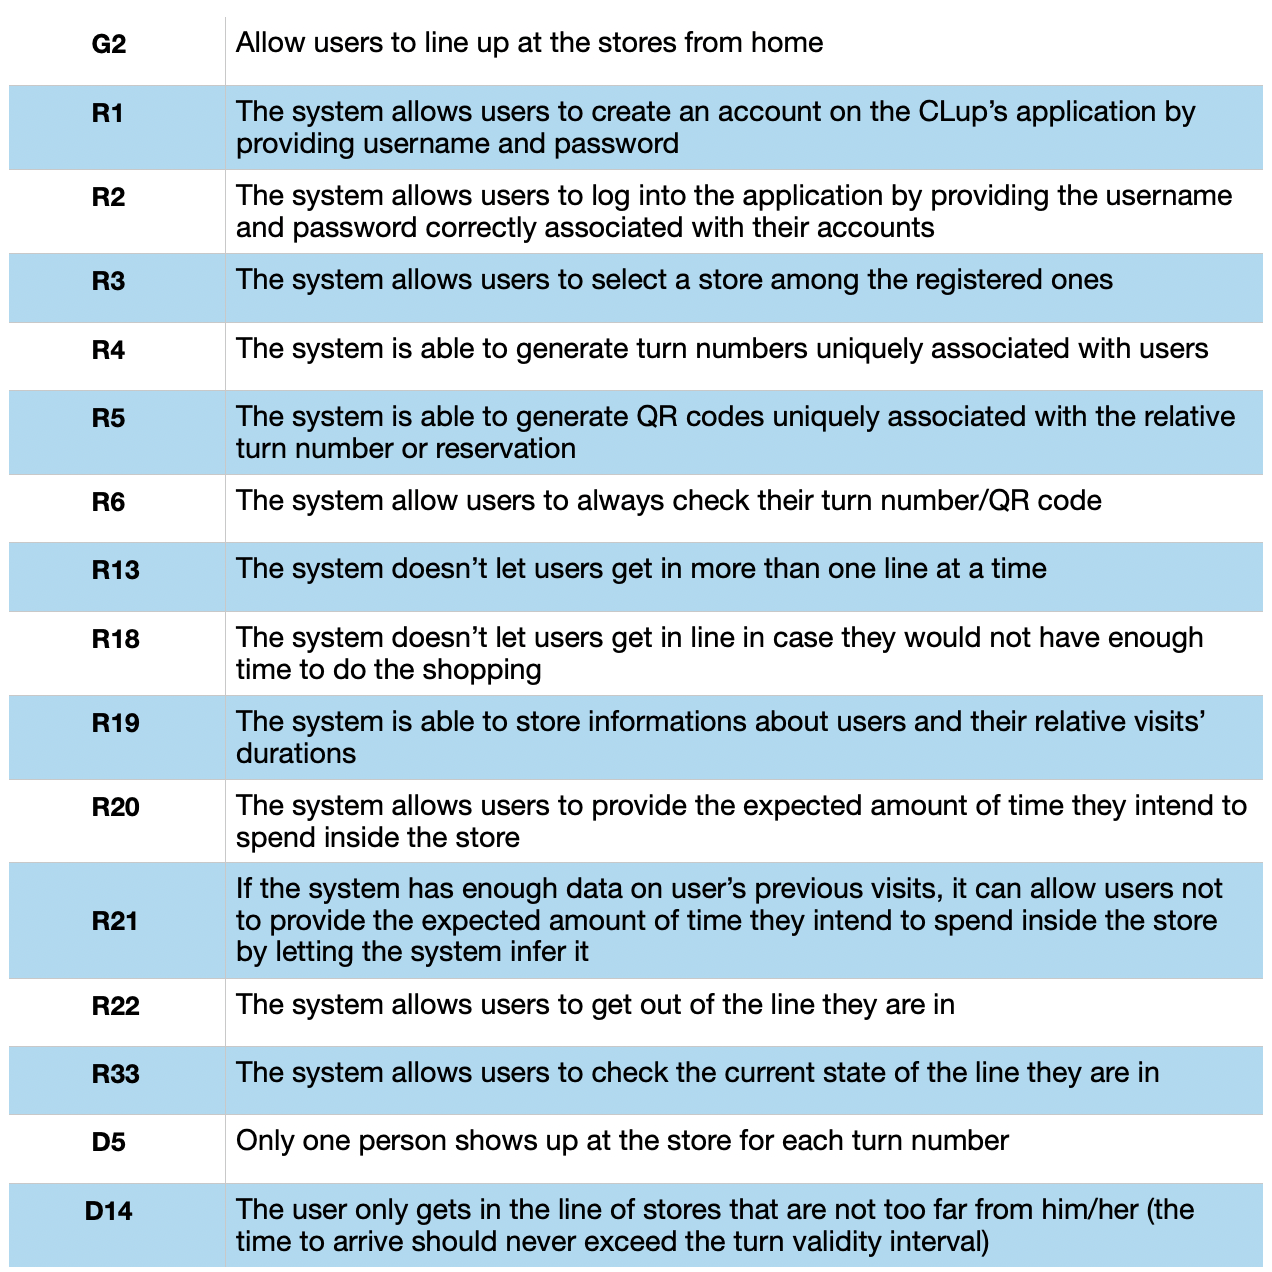
\includegraphics[width=\linewidth]{Mapping2.png}
  
\end{figure}

\begin{figure}[H]
  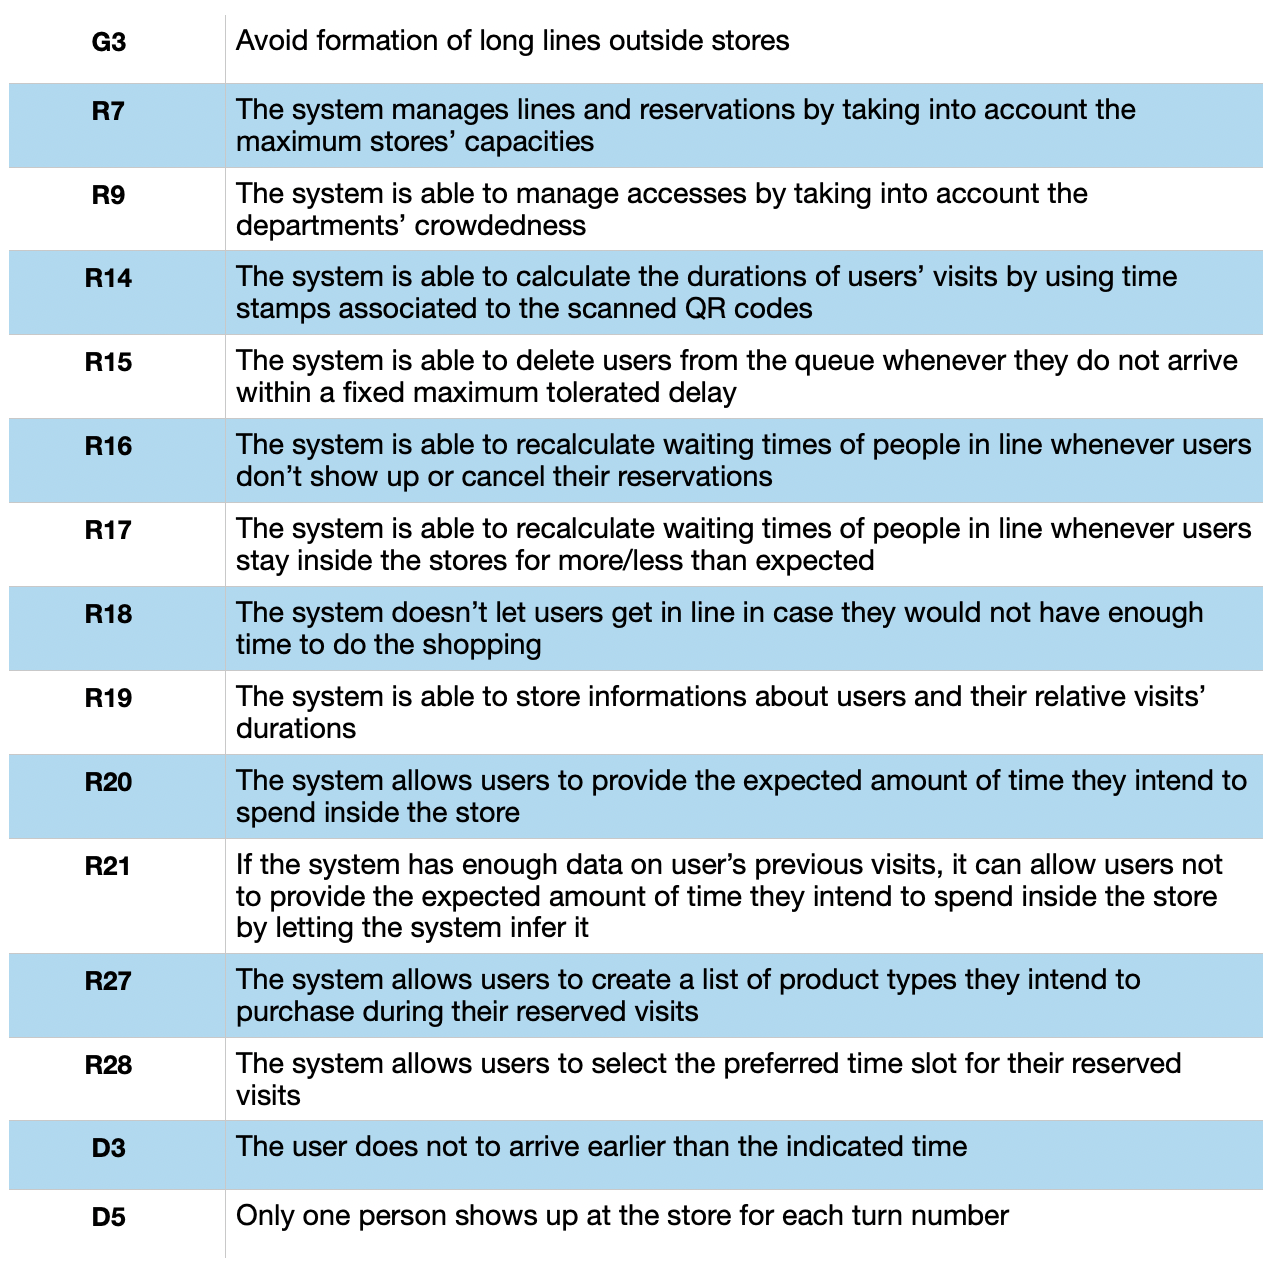
\includegraphics[width=\linewidth]{Mapping3.png}
  
\end{figure}

\begin{figure}[H]
  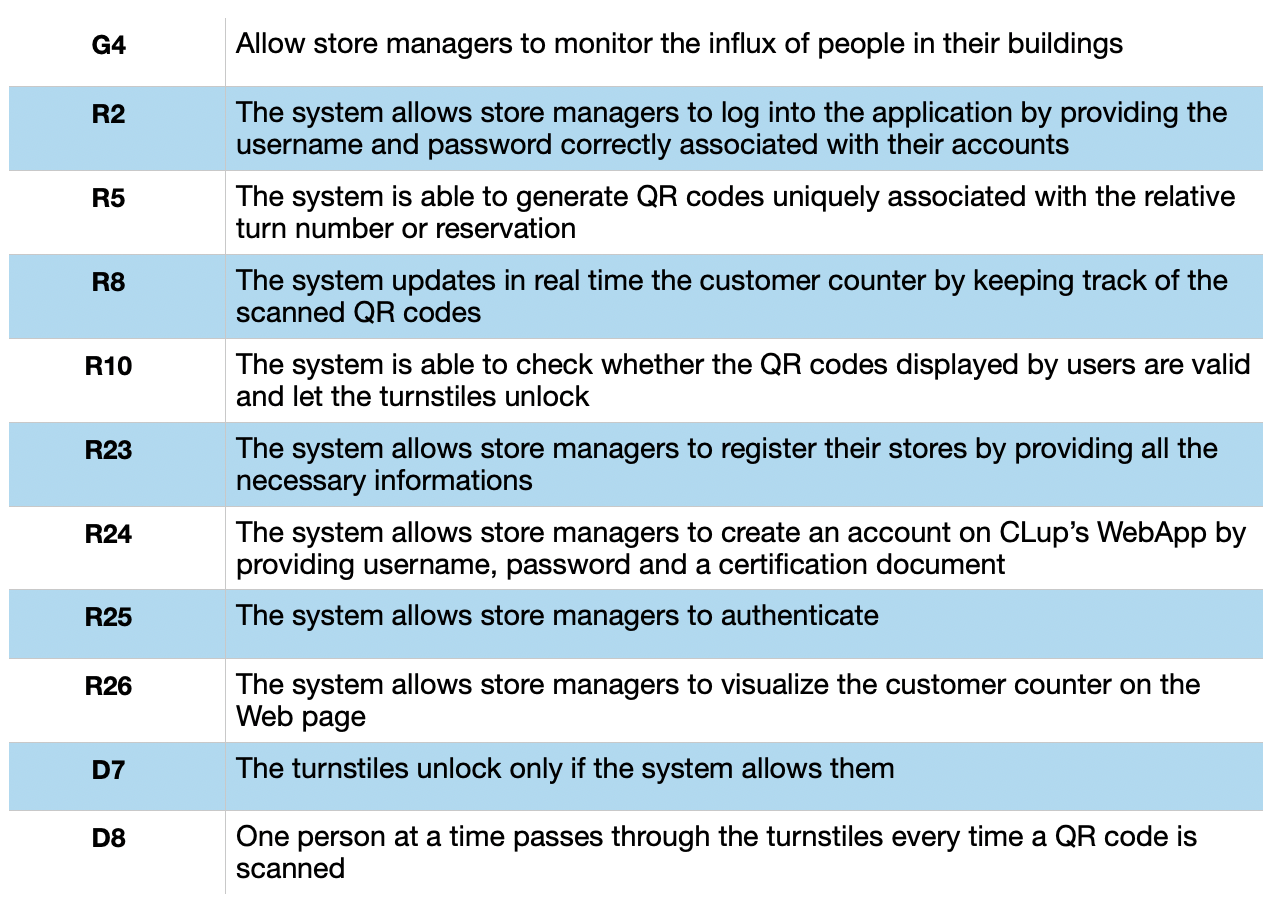
\includegraphics[width=\linewidth]{Mapping4.png}
  
\end{figure}

\begin{figure}[H]
  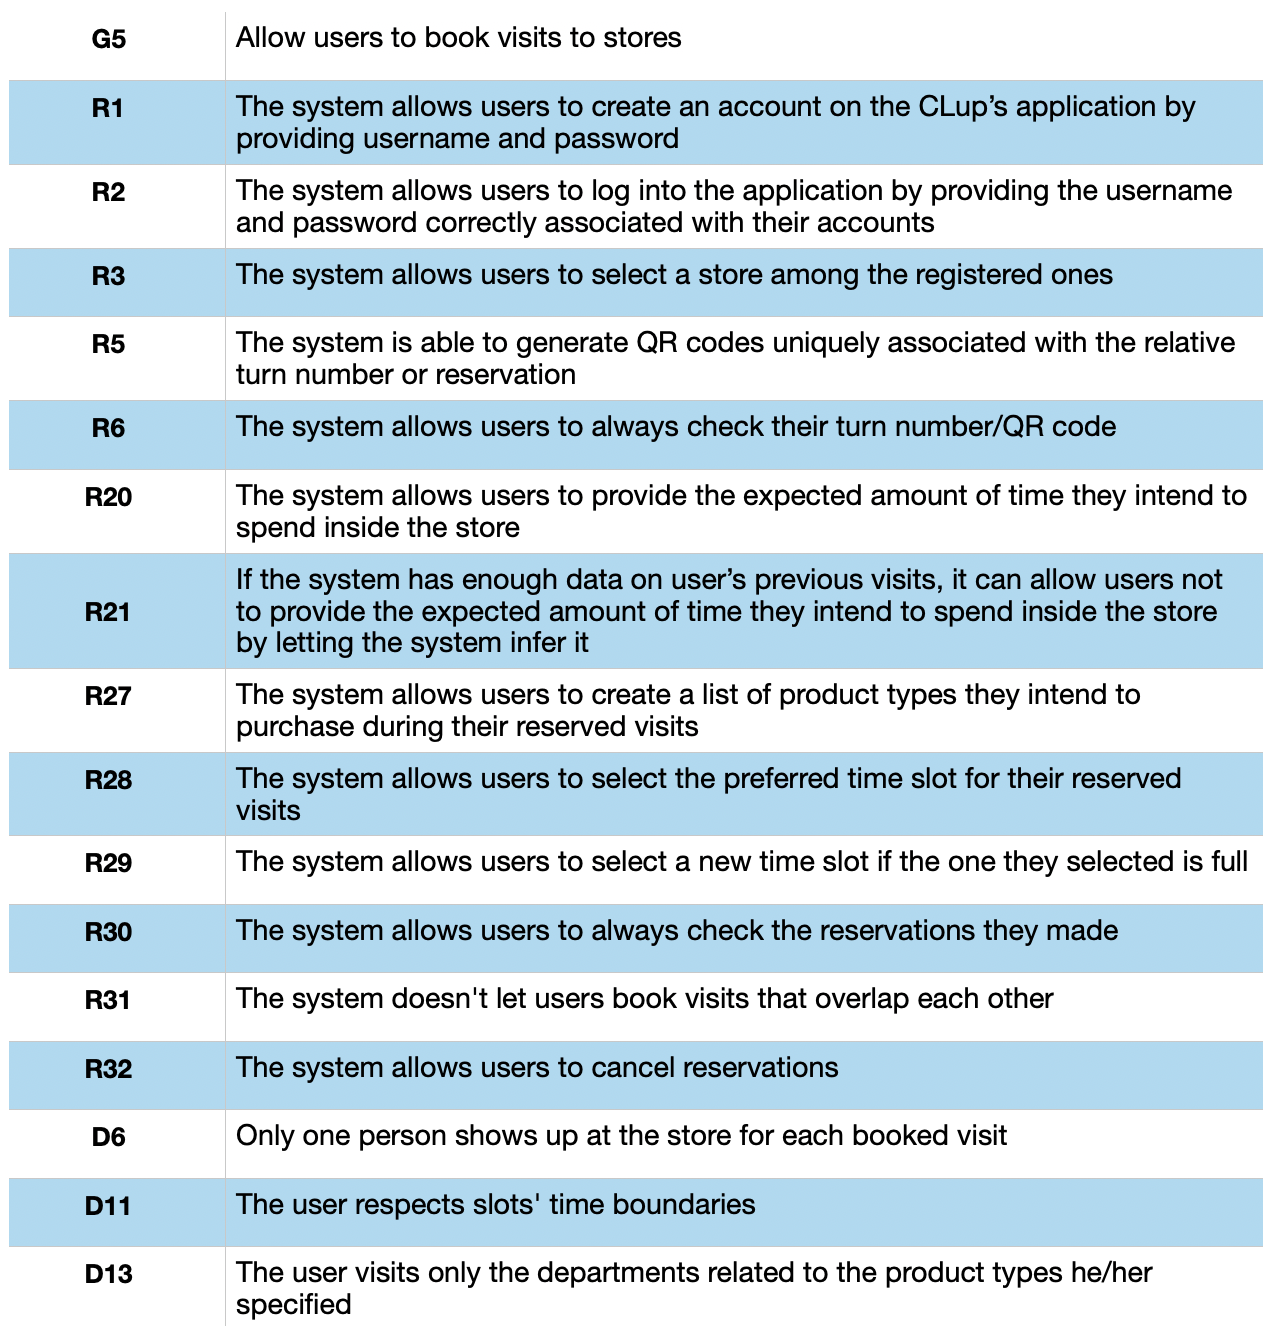
\includegraphics[width=\linewidth]{Mapping5.png}
  
\end{figure}

\begin{figure}[H]
  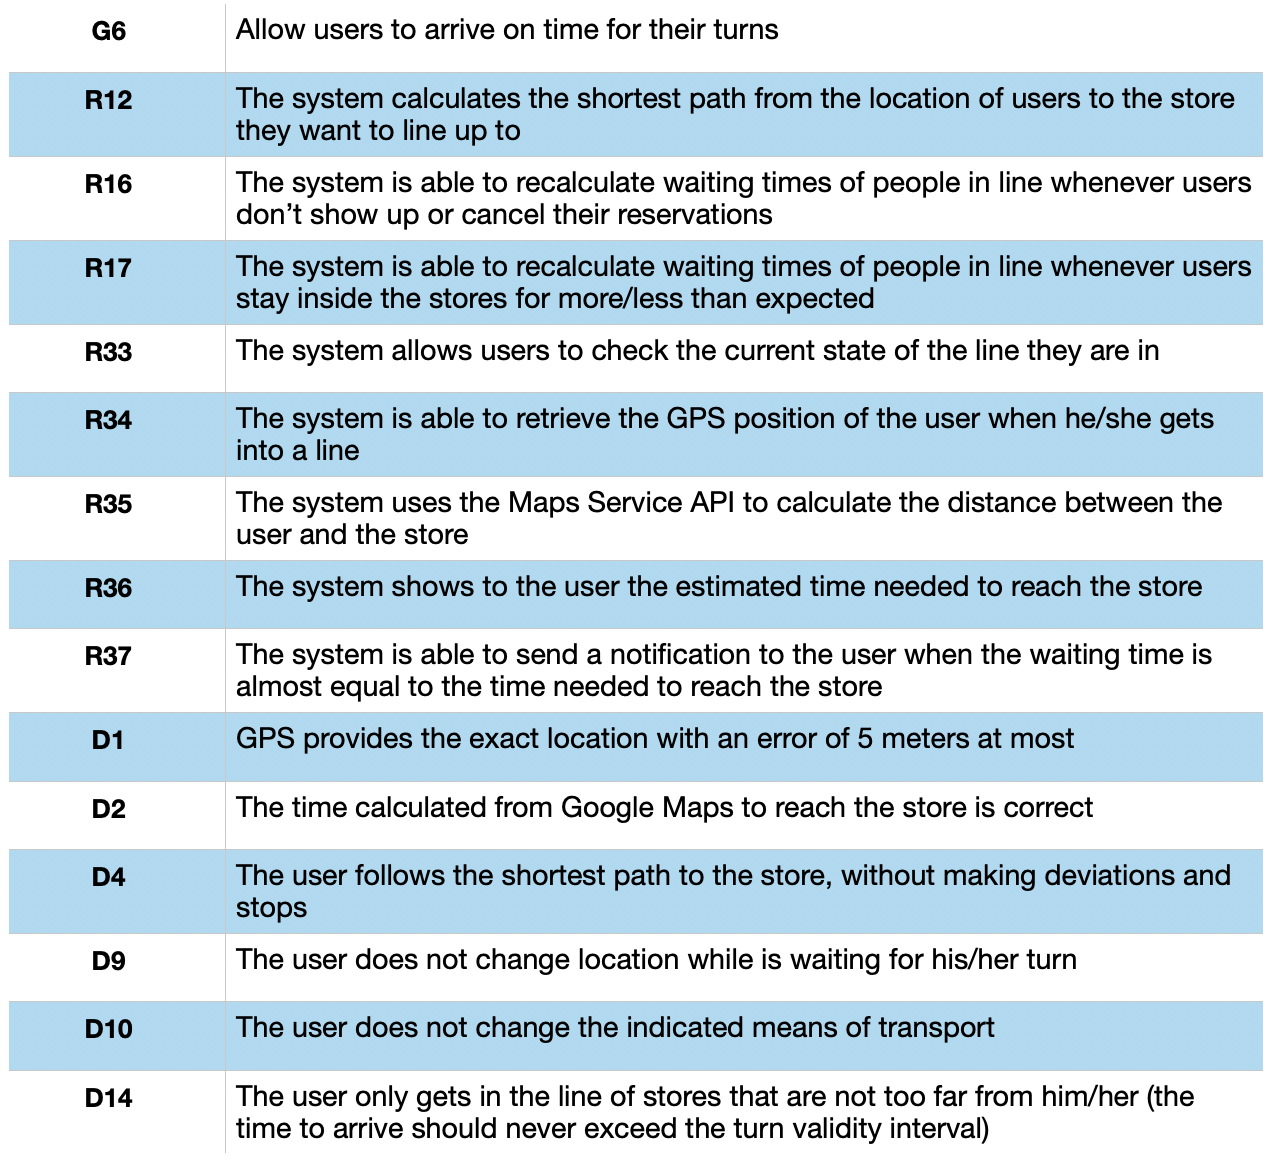
\includegraphics[width=\linewidth]{Mapping6.png}
  
\end{figure}


\subsubsection{Scenarios}
\medskip
\textbf{Scenario 1: Line up}\medskip\\
Mario is a 40 years old teacher living in Pisa. During the weekend, he wants to take advantage of some free time to go grocery shopping for the coming week. Since the covid-19 pandemic is getting worse, he does not want to risk ending up in crowded lines or stores. Therefore, he decides to exploit the virtual lining service, offered by CLup application on his smartphone. He chooses the nearest Eurospin on the app and finds out that the waiting time is 40m 32s. He decides to get in line and selects “on foot” as means of transport, to get some fresh air. He wants to do a lot of shopping, so he indicates an hour as estimated time to spend inside the store. After approximately 15 min, Mario receives a notification from CLup saying that it’s time to leave and therefore, he prepares for his 20 min walk to reach the store. Once arrived, he sees his number on the board, he selects the QR code on his smartphone to have it scanned by the turnstile at the entrance and, finally, he starts shopping.\medskip\\
\medskip
\textbf{Scenario 2: Get out of line}\medskip\\
Elisa is a young mum of two kids who decides to go shopping for Christmas’ presents on a Wednesday morning, while her children are at school. Considering that Christmas is coming, she expects to find many people shopping and so she decides to use the CLup application to get in the line of her favorite gift shop. The current waiting time is such that she will be perfectly in time to pick her kids up from school. Unfortunately, it seems like some store’s departments are particularly crowded, or maybe some customers are staying inside more than they should. As a result, Elisa’s waiting time has increased a little and she realizes she would be late for the end of school. In the end, she gets out of the line and decides to try again the following day. \medskip\\
\medskip
\textbf{Scenario 3: Book a visit}\medskip\\
Anna is a single 36 years old business woman currently living in Milan. She has a very busy schedule and therefore she cannot risk wasting too much time buying groceries. For this reason, she often uses CLup application on her smartphone to book visits to her usual supermarket. On Tuesday, she will be getting off work at 4 pm and she has exactly two hours, before a late afternoon video call. Among the available time slots, she chooses the one from 5:30 pm till 6:30 pm, as she is sure she will not need to stay inside for more than half an hour. Last time she went to the supermarket, it took her 20 min to do the shopping, so she selects that same duration, shown by the system, for her Tuesday’s visit as well. Lastly, she select the categories of products that she intends to purchase and confirms the whole reservation.\medskip\\
\medskip
\textbf{Scenario 4: Cancel a reservation}\medskip\\
Giorgio is a young man working as a consultant in Turin. While he’s in the office, he decides to make a reservation to go to the supermarket later in the afternoon, because he wants to surprise his wife with the grocery. He uses CLup application to book the visit for the preferred time slot. At lunch time, Giorgio’s wife, who does not trust her husband’s sense of initiative, calls Giorgio to inform him that she is going grocery shopping. At this point, the poor Giorgio is forced to cancel his booked visit. He opens CLup app, goes in the “My Reservations” section and cancels his last reservation.\medskip\\
\medskip
\textbf{Scenario 5: Customer without a smartphone gets a ticket}\medskip\\
Antonio is a 71 years old retired man who lives in Monza during the period of lockdown, due to the COVID-19 pandemic. Antonio is reluctant to technology and in fact, the cellphone he owns is suitable only for basic functionalities. For this reason, he is not able to download CLup’s application and use its services. He needs to go grocery shopping, so he walks up to the nearest supermarket. He reaches the info desk and finds out that there is a virtual lining mechanism going on and that he will have to wait for his turn at the entrance. Angela, a store’s employee who is responsible for taking care of customers who do not have access to the required technology, accesses to CLup’s WebApp from her computer and prints for Antonio a ticket, with a turn number and a QR code. She explains to him how and where to scan the QR code as soon as his turn number appears on the led board at the entrance.\medskip\\
\medskip
\textbf{Scenario 6: Check customer counter}\medskip\\
Paola is the manager of a big Esselunga store in Milan. During the day, she periodically checks that everything is proceeding as planned. In particular, she takes a look at each store department to make sure that there are no crowds and she also checks the number of people currently in the store. To do so, she accesses CLup’s WebApp from her office’s computer and clicks on “Check customer counter” button. In this way, she is always able to verify whether the CLup system is efficiently working, without violating the maximum capability of her store.\medskip\\

\subsubsection{Use Cases Diagram}

\begin{figure}[H]
  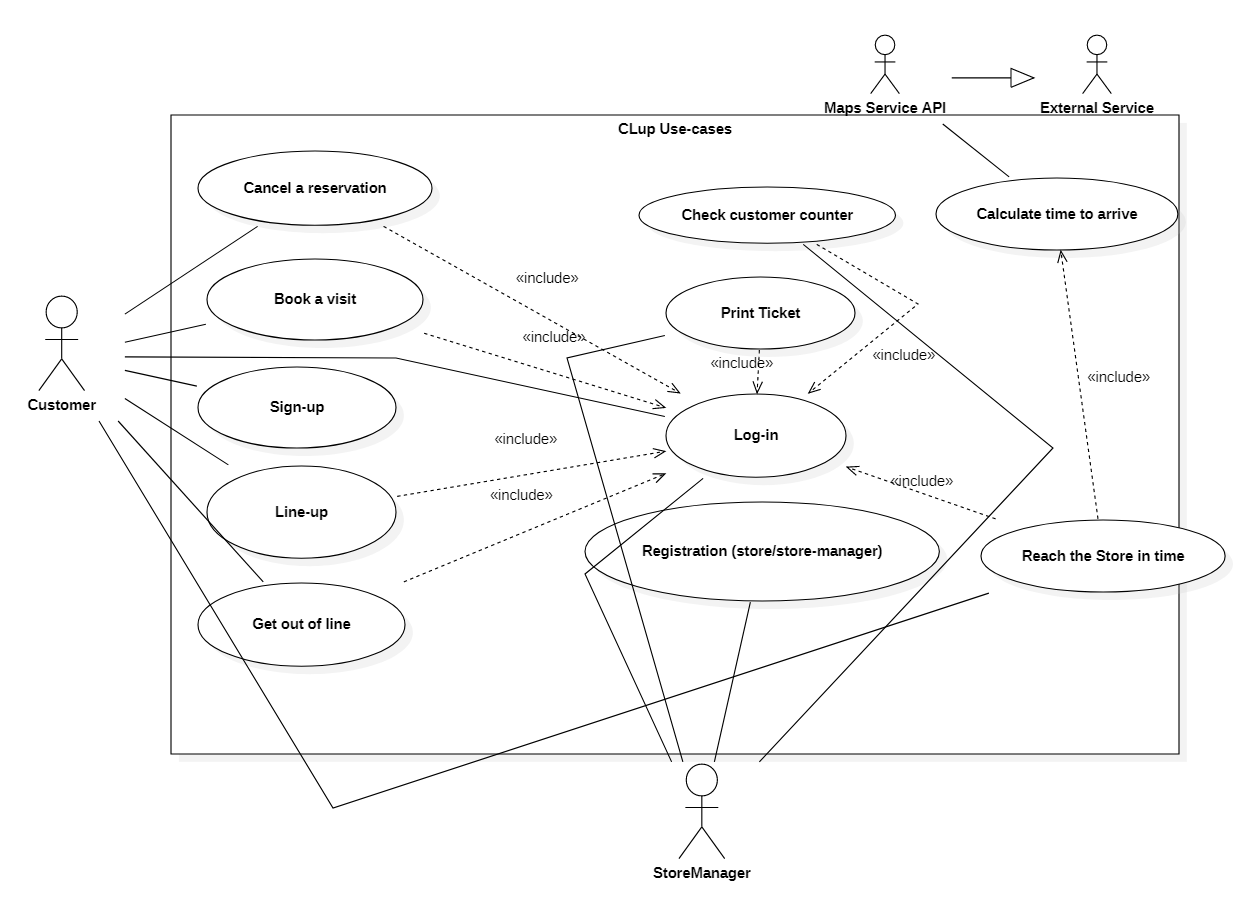
\includegraphics[width=\linewidth]{useCasesDiagram.png}
  
\end{figure}

\subsubsection{Use Cases}

\begin{figure}[H]
  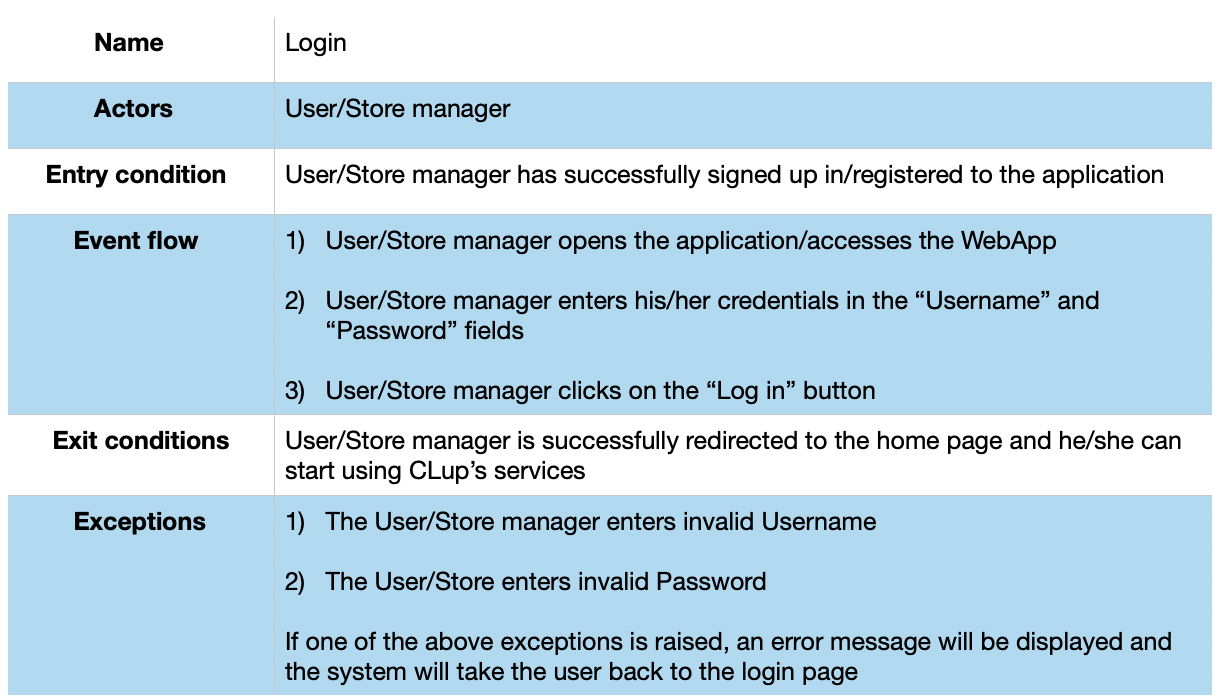
\includegraphics[width=\linewidth]{LoginUseCase.png}
  
\end{figure}

\begin{figure}[H]
  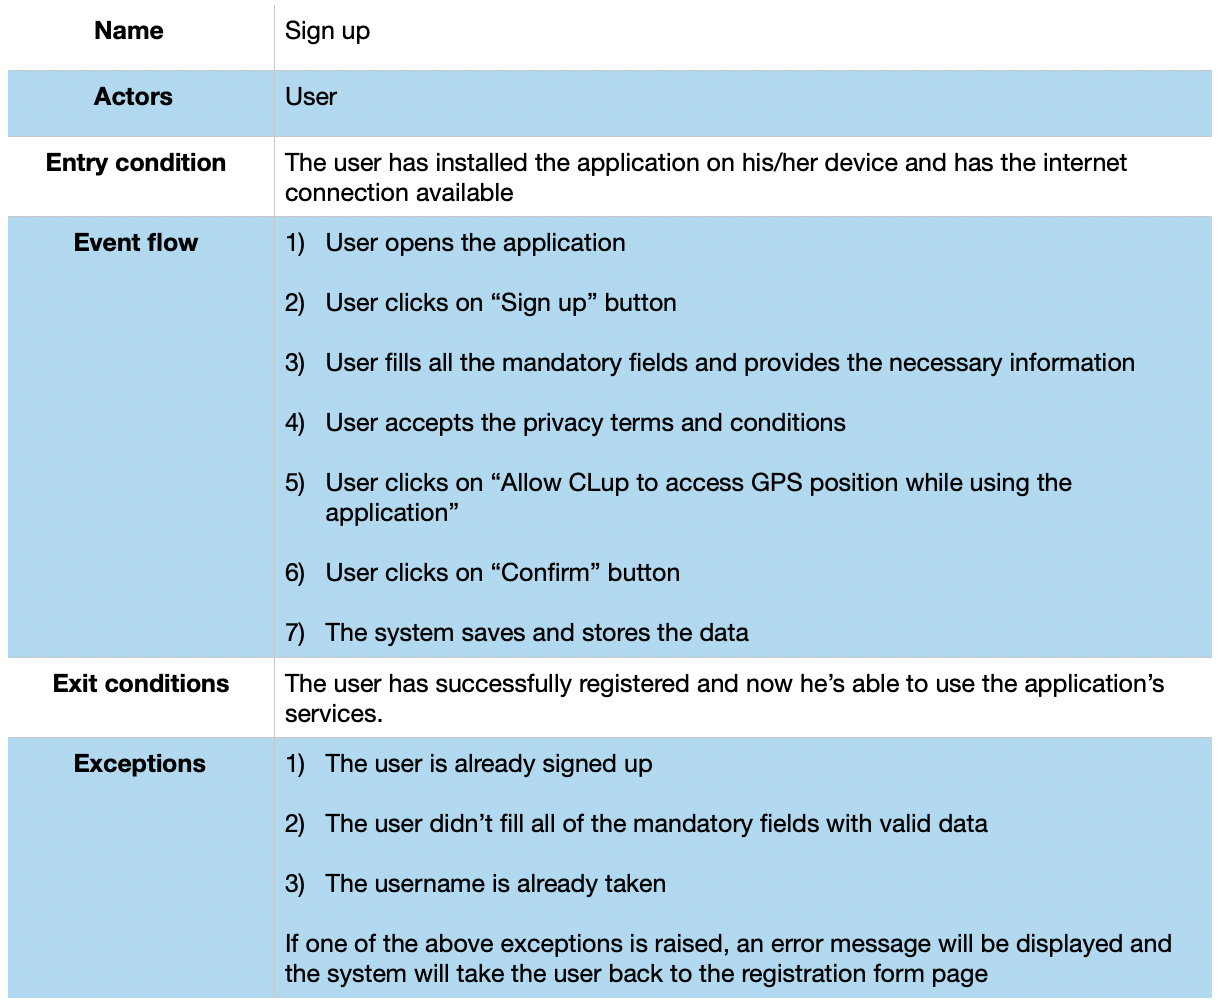
\includegraphics[width=\linewidth]{SignUpUseCase.png}
  
\end{figure}

\begin{figure}[H]
  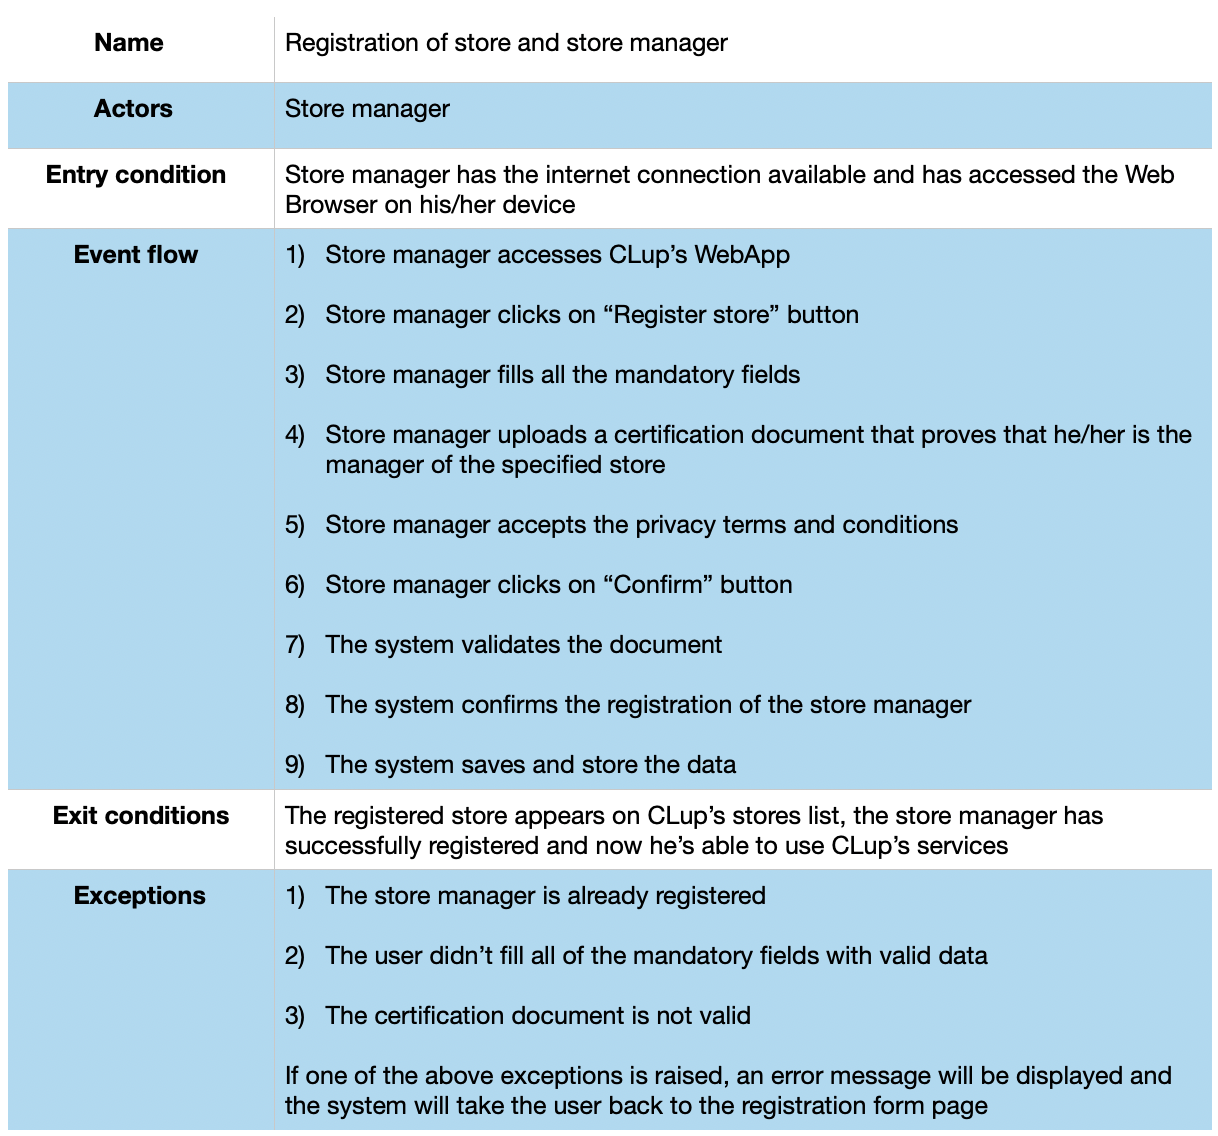
\includegraphics[width=\linewidth]{RegistrationStoreUseCase.png}
  
\end{figure}

\begin{figure}[H]
  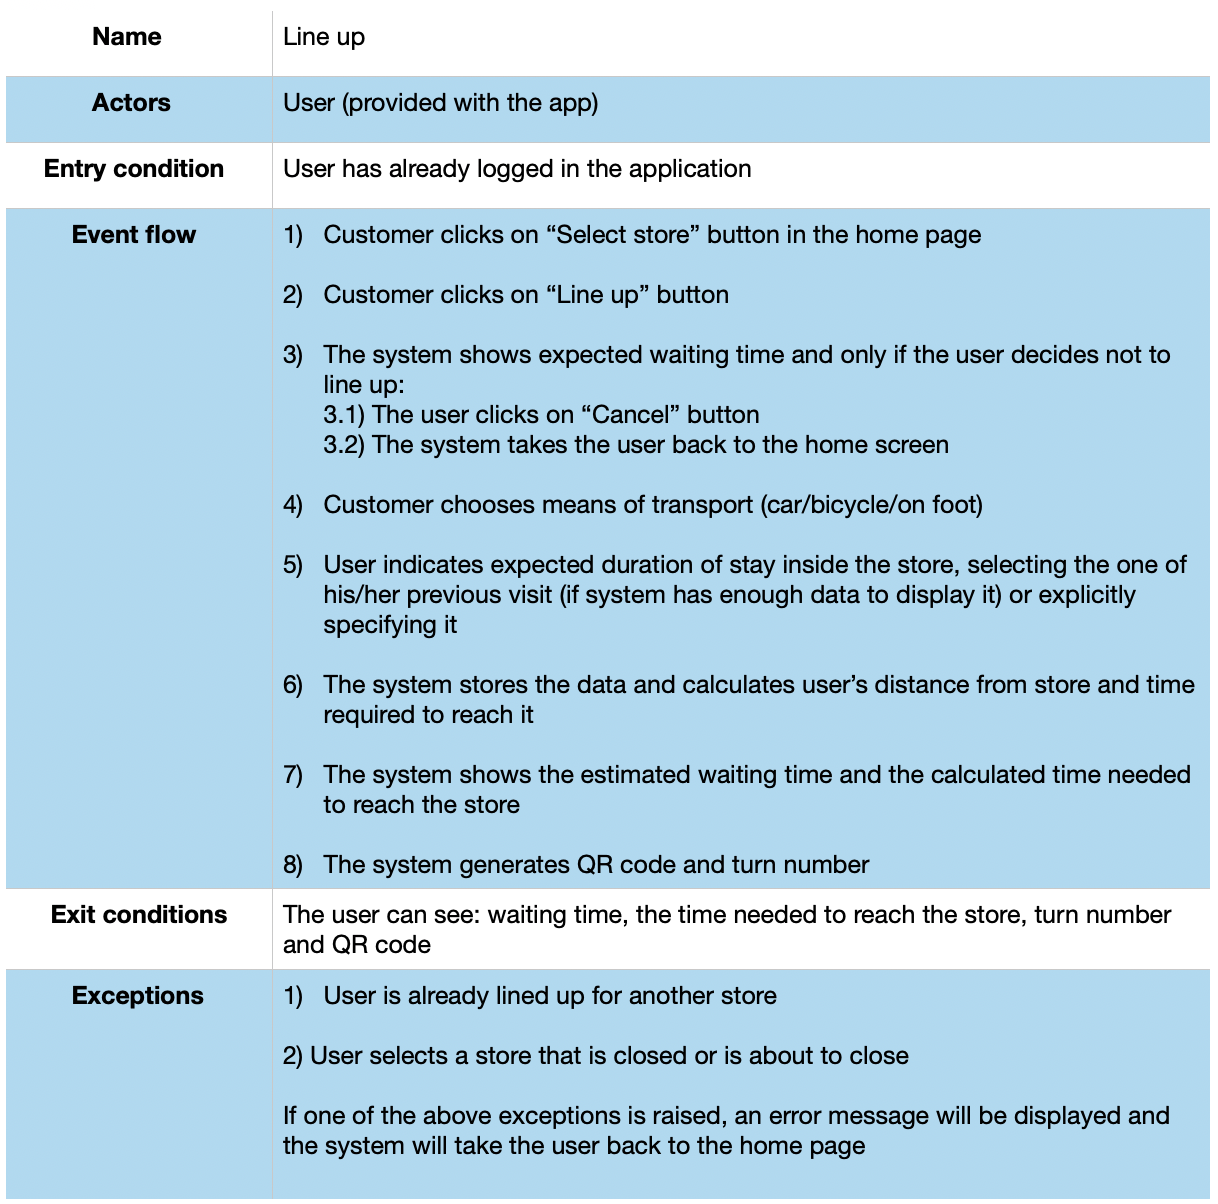
\includegraphics[width=\linewidth]{LineUpUseCase.png}
  
\end{figure}

\begin{figure}[H]
  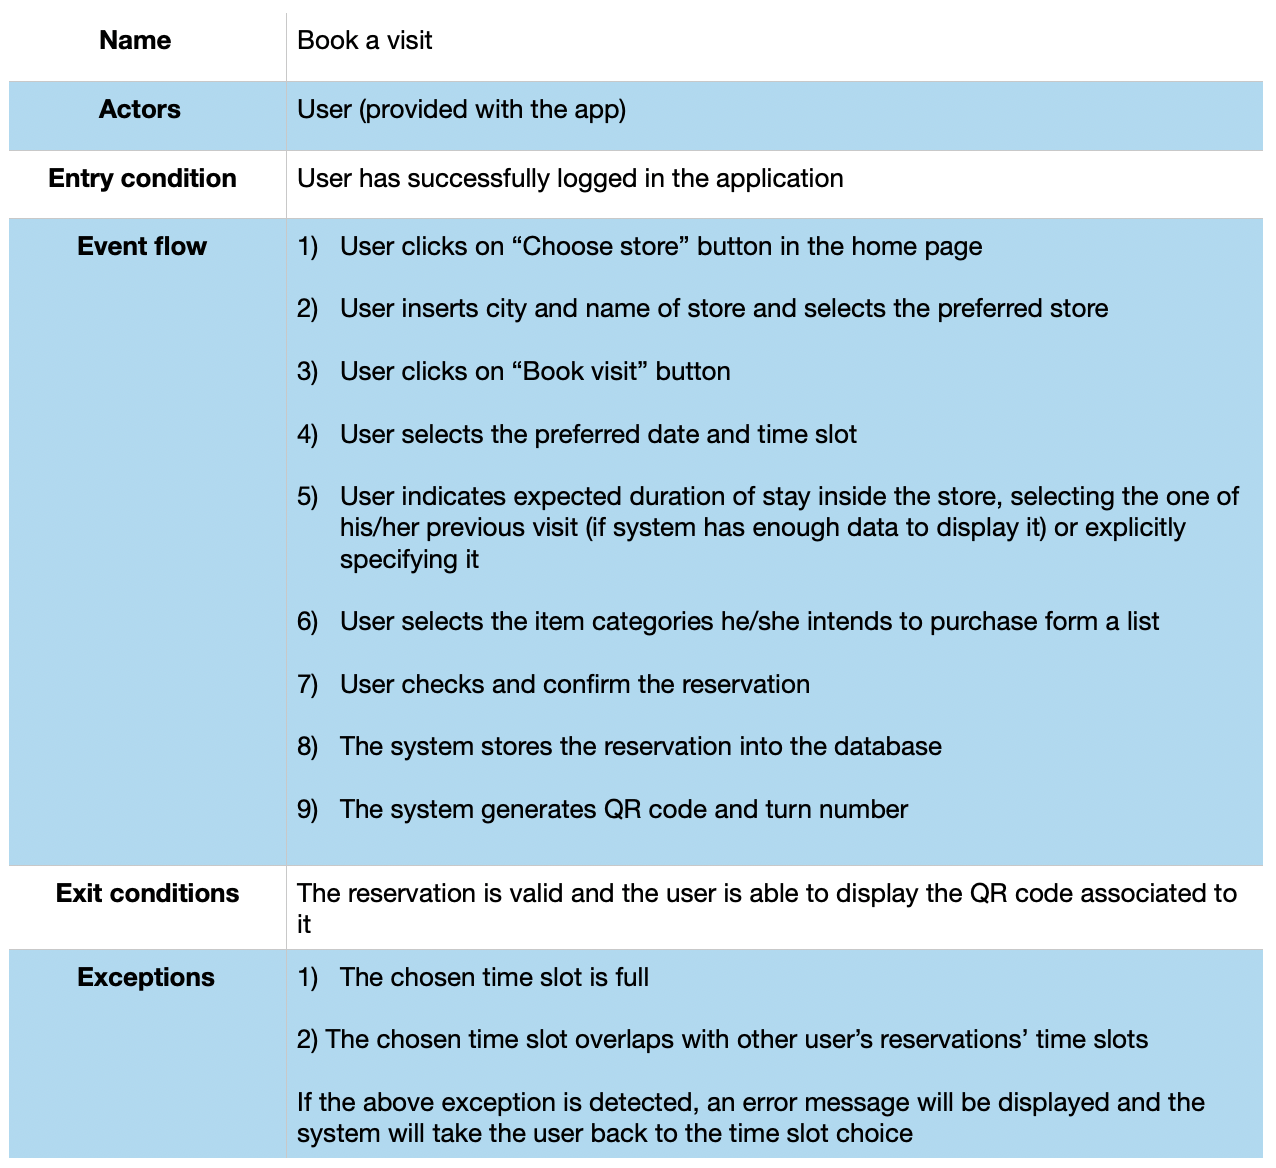
\includegraphics[width=\linewidth]{BookVisitUseCase.png}
  
\end{figure}

\begin{figure}[H]
  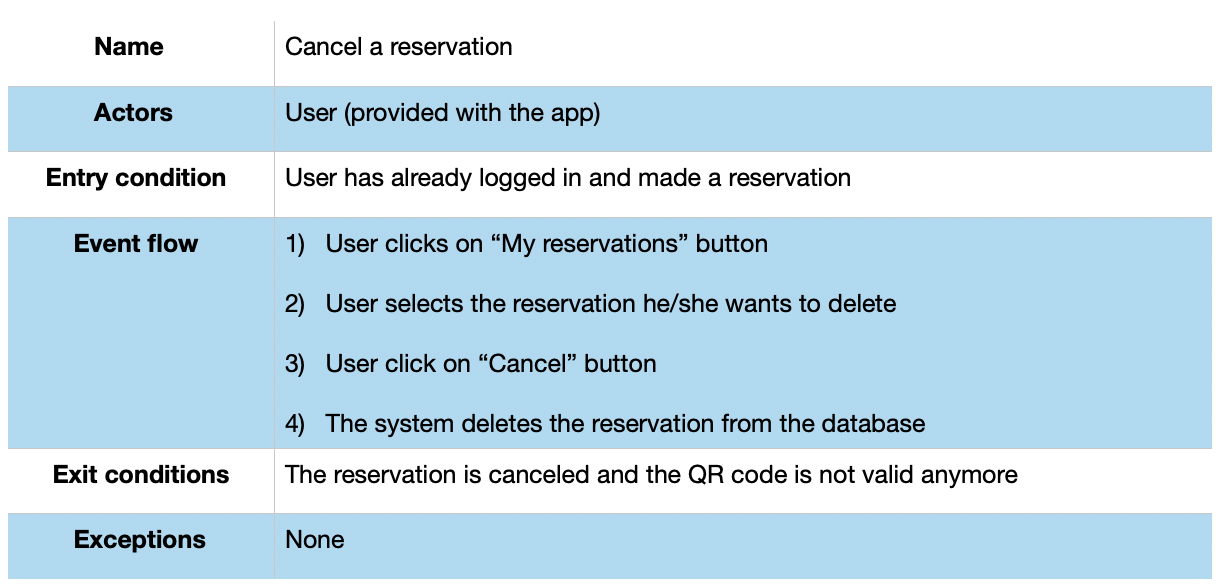
\includegraphics[width=\linewidth]{CancelReservationUseCase.png}
  
\end{figure}

\begin{figure}[H]
  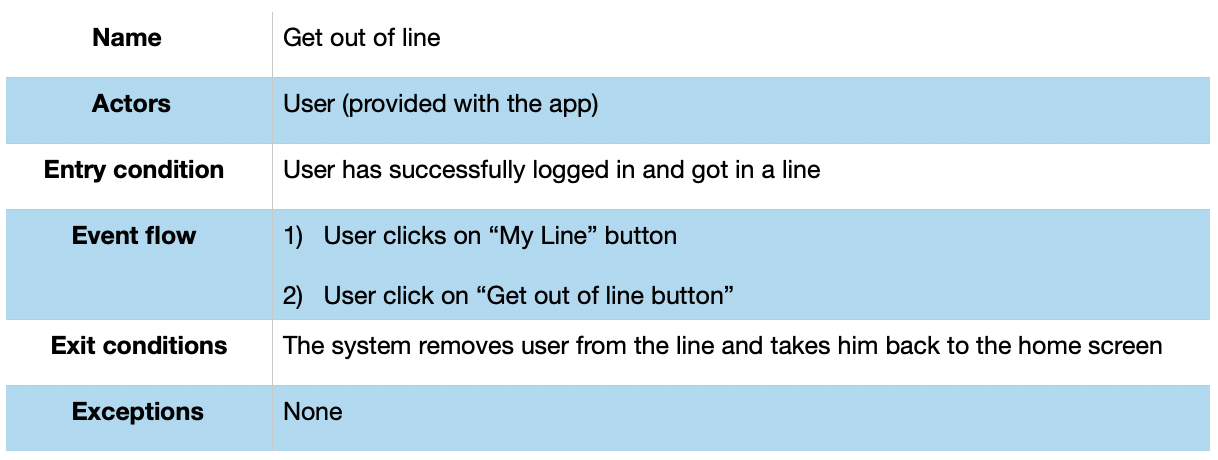
\includegraphics[width=\linewidth]{GetOutLineUseCase.png}
  
\end{figure}

\begin{figure}[H]
  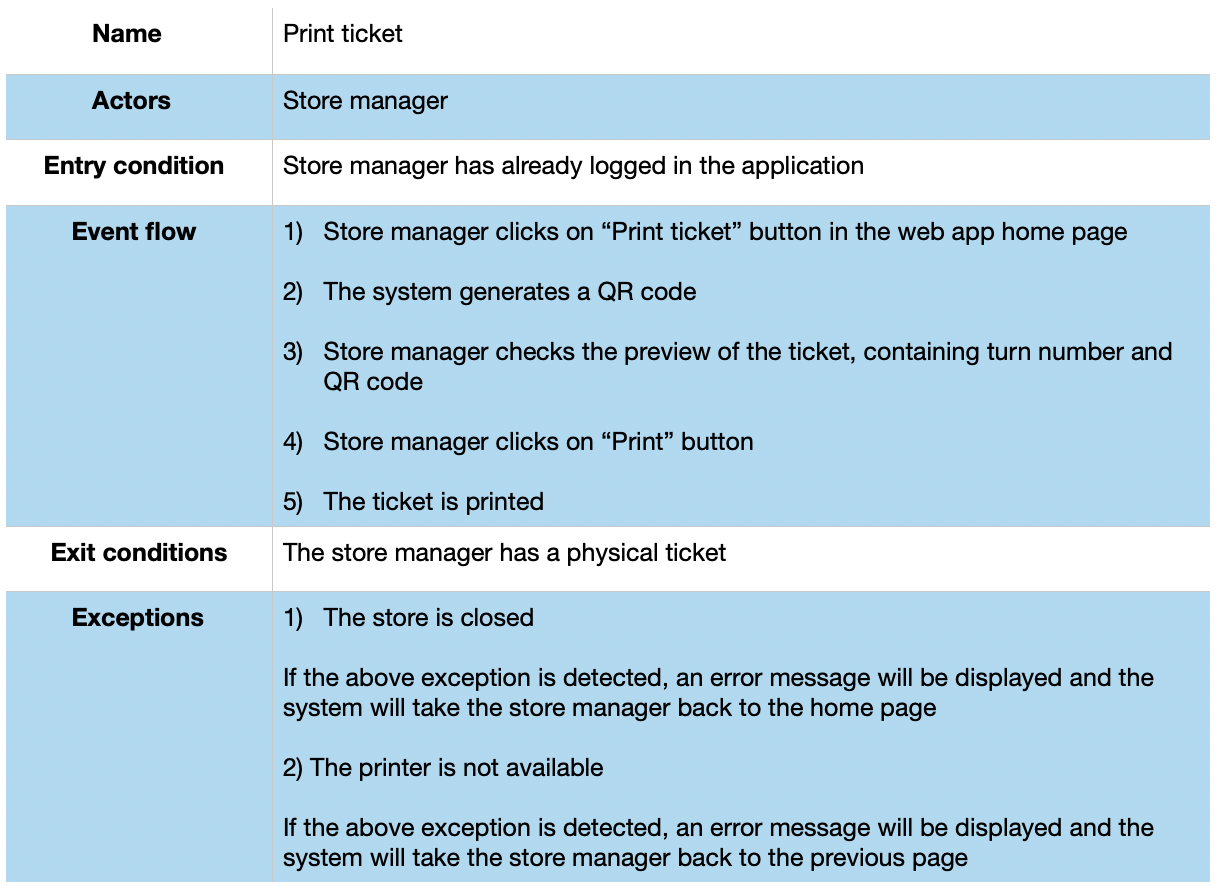
\includegraphics[width=\linewidth]{PrintTicketUseCase.png}
  
\end{figure}

\begin{figure}[H]
  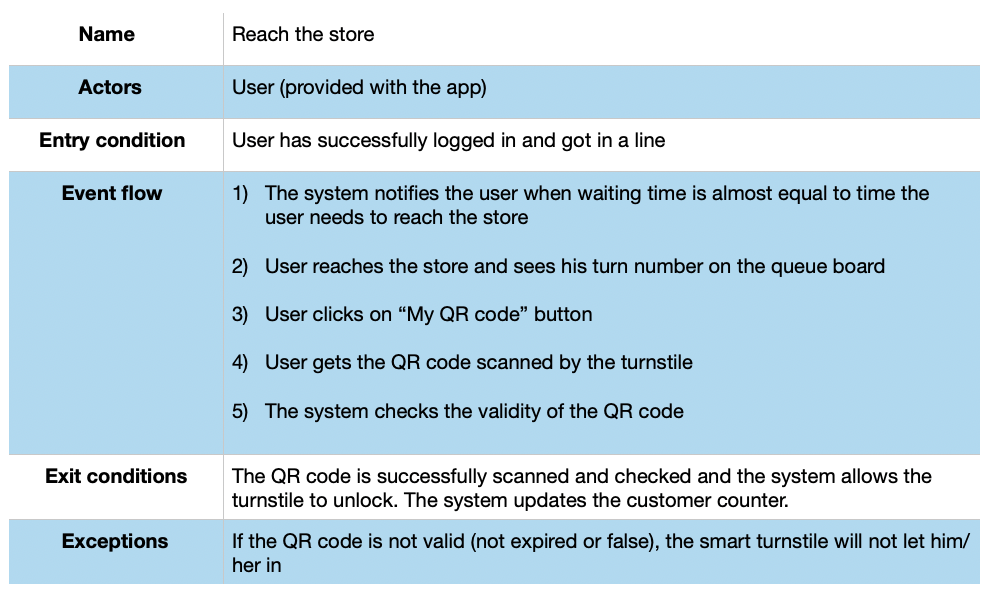
\includegraphics[width=\linewidth]{ReachStoreUseCase.png}
  
\end{figure}

\begin{figure}[H]
  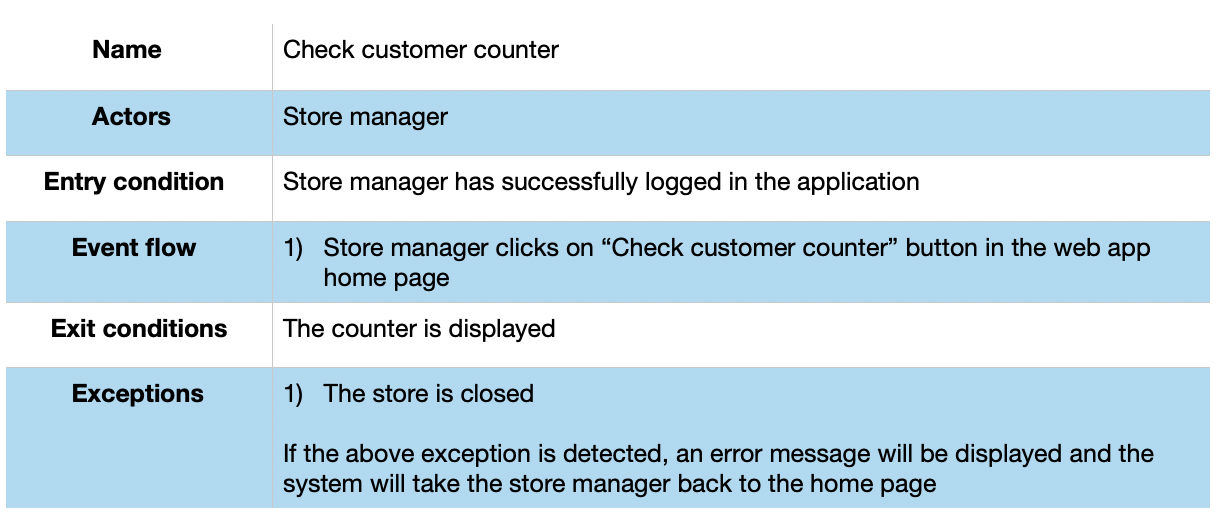
\includegraphics[width=\linewidth]{CheckCustomerCounterUseCase.png}
  
\end{figure}

\subsubsection{Sequence Diagrams}

\begin{figure}[H]
  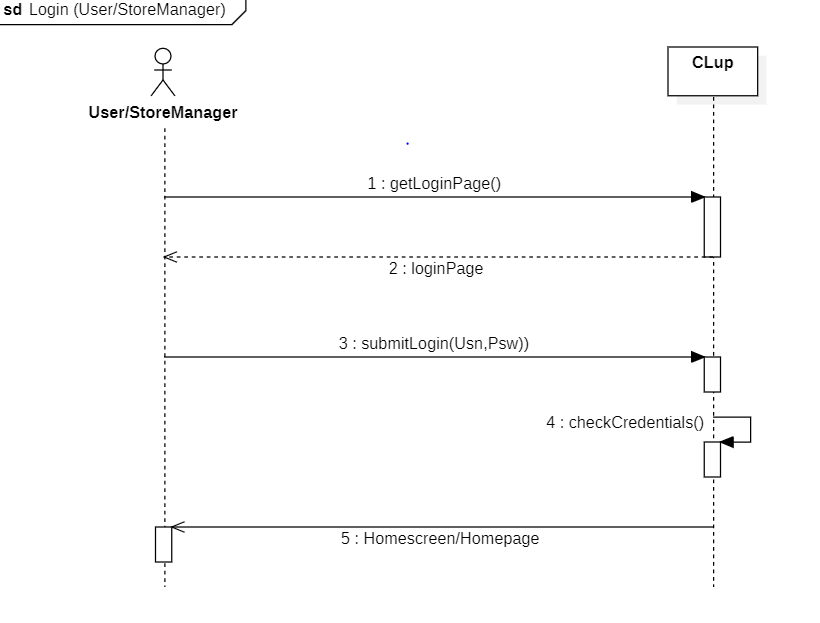
\includegraphics[width=\linewidth]{LoginSequence.png}
  
\end{figure}

\begin{figure}[H]
  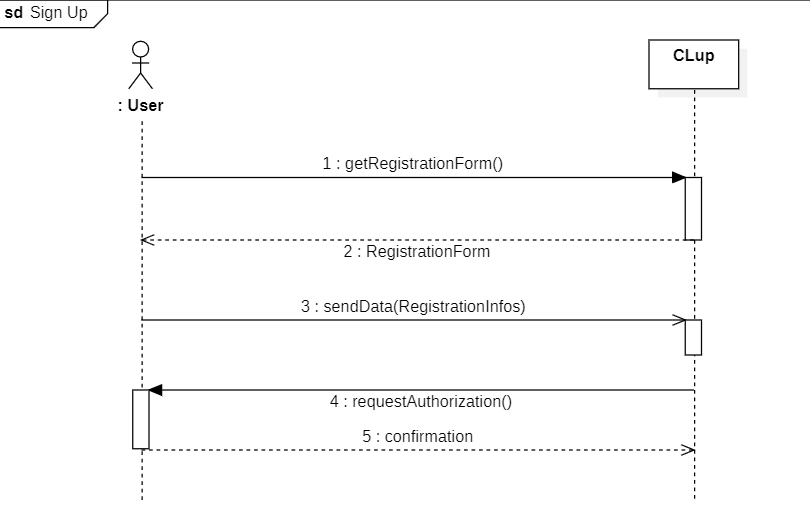
\includegraphics[width=\linewidth]{SignUpSequence.png}
  
\end{figure}

\begin{figure}[H]
  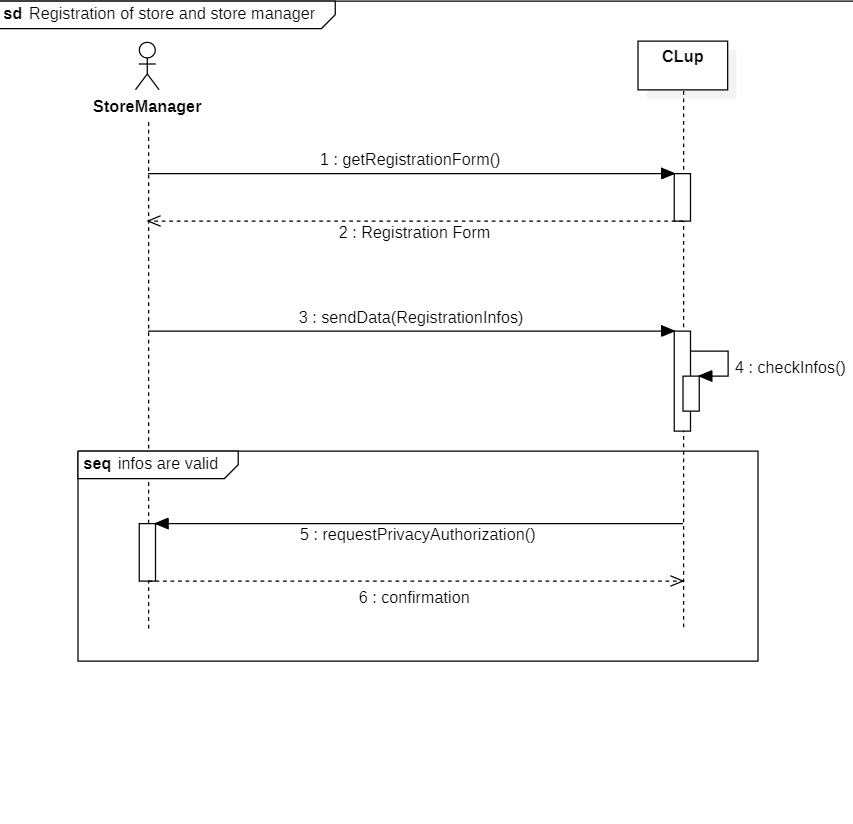
\includegraphics[width=\linewidth]{RegistrationSequence.png}
  
\end{figure}

\begin{figure}[H]
  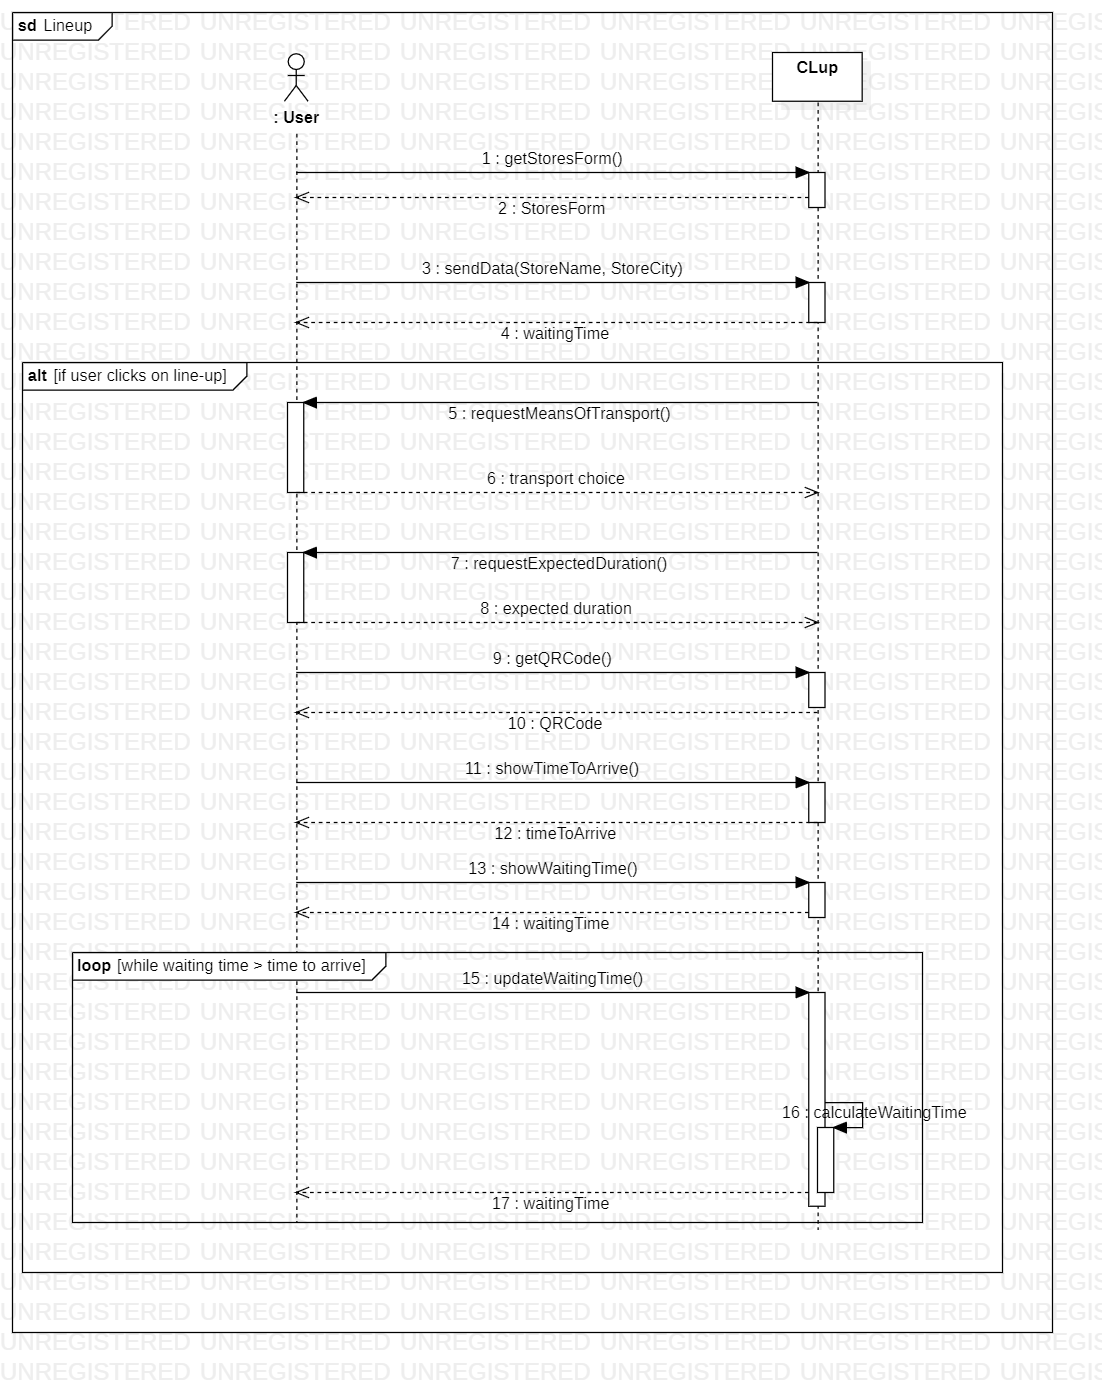
\includegraphics[width=\linewidth]{LineUpSequence.png}
  
\end{figure}

\begin{figure}[H]
  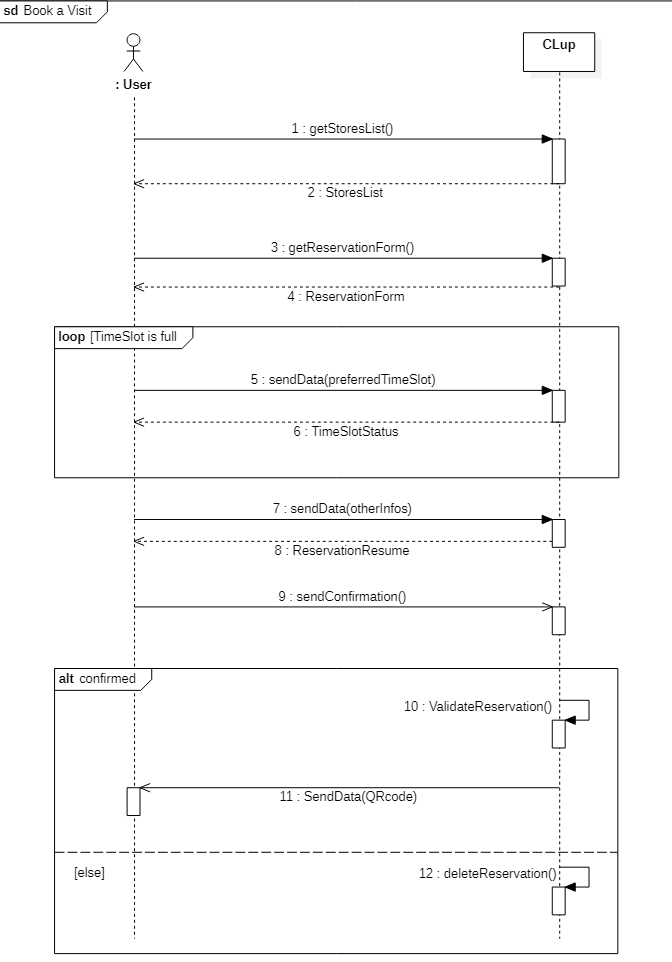
\includegraphics[width=\linewidth]{BookSequence.png}
  
\end{figure}

\begin{figure}[H]
  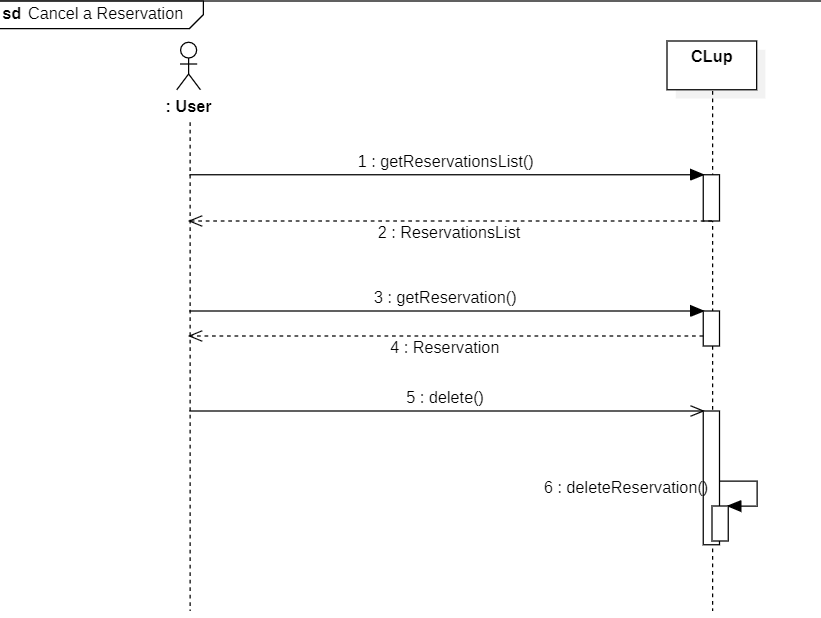
\includegraphics[width=\linewidth]{CancelReservationSequence.png}
  
\end{figure}

\begin{figure}[H]
  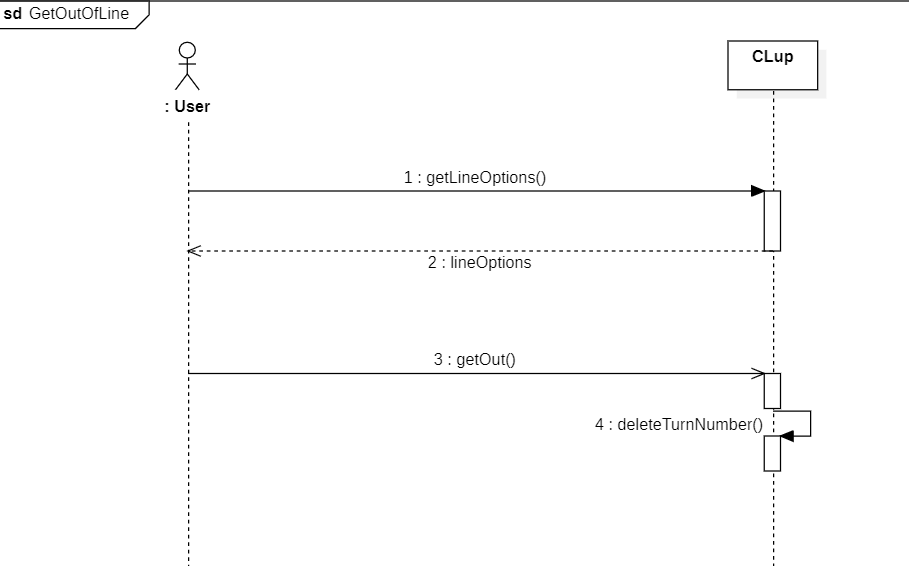
\includegraphics[width=\linewidth]{OutOfLineSequence.png}
  
\end{figure}

\begin{figure}[H]
  \includegraphics[width=\linewidth]{PrintTicketSequence.png}
  
\end{figure}

\begin{figure}[H]
  \includegraphics[width=\linewidth]{ReachStoreSequence.png}
  
\end{figure}




\subsection{Performance Requirements - Non-functional Requirements}
It is important to remark that the CLup system provides services that help people to avoid risks and to respect the limitations imposed by the coronavirus emergency. For this reason, the system has to be able to serve a great number of users and store managers simultaneously. The system also has to be able to update the waiting times seen by the users in a quick, reactive and correct way, as soon as they change in the system’s database.

\subsection{Design Constraints - Non-functional Requirements}
\subsubsection{Hardware limitations}
The hardware requirements needed in order to use the system’s functionalities on the mobile app are the following:
\begin{itemize}
\item iOS or Android smartphone 
\item GPS
\item Connection to internet (Wi-Fi/4G/3G/2G) 
\end{itemize}
\subsubsection{Any other constraints}
The system will have to ask users' permission to retrieve and use their positions without storing them. Moreover, the collection and treatment of personal data must comply with the principles and rules of the General Data Protection Regulation (GDPR).

\subsection{Software System Attributes - Non-functional Requirements}
\subsubsection{Reliability and Availability}
The system must guarantee a 24/7 service. It is expected to be available 99.99\% of the time, considering the critical situation due to the coronavirus pandemic.
\subsubsection{Security}
Passwords and sensitive informations like the recordings of users' durations of visits must be protected using encryption.
\subsubsection{Maintainability}
The development of the application must guarantee a high level of maintainability and flexibility, in order to make the addiction of new features and options easy and cheap. For this reason, appropriate design patterns will be used, which will be detailed in an adequate document.
\subsubsection{Scalability}
The system is expected to be built considering a high level of scalability on the number of stores (and therefore the number of users).
\subsubsection{Compatibility}
The WebApp must be compatible with the most popular browsers, while the smartphone application must be compatible with Android Oreo or later versions and on iOs 11 or later versions in order to be available on a wide range of devices.


\section{Formal Analysis Using Alloy}

In this section we present our alloy code and results. We decided to focus on some relevant system's aspects with the aim to model these constraints:
\begin{itemize}
\item A notification is shown to a lined-up user if waiting time approaches time to arrive
\item No overlaps between same user's reservations
\item Every QRcode is associated to only one reservation or turn number
\item In a queue, waiting time related to a turn number is <= waiting time related to the next turn numbers
\item A store's counter can't exceed store's capacity

\end{itemize}
To simplify alloy modelling we decided to show the notification if "waiting time" is equal to the "time to arrive", even if in the real application the notification is shown when one is approaching the other (with a delta of few minutes).

\begin{lstlisting}[language=alloy]

open util/integer


sig Time {
    minutes: one Int
}

{ minutes >= 0 }

sig Date { }

sig Location {
	timeToArrive: one Time
}
{
	timeToArrive.minutes>0
}

sig QRcode { }

sig User { 
    reservations: set Reservation,
    turnNumber: lone TurnNumber,
    notification: lone Notification,
    queue: lone Queue
}

sig Notification {
	user: one User
}

sig TurnNumber {
    
    user: one User,
    qrCode: one QRcode,
    number: one Int,
    location: one Location,
    queue: one Queue,
    waitingTime: one Time,
    

 }{
     
     number>0 and
     (waitingTime.minutes >= 0) and
     (location.timeToArrive.minutes >= 0) and
     (waitingTime.minutes >= location.timeToArrive.minutes) 
      
 }

sig Reservation {

    startTime: one Time,
    endTime: one Time,
    date: one Date,
    user: one User,
	duration: one Int,
    qrCode: one QRcode
}{

(sub[endTime.minutes, startTime.minutes] >= duration) and
(startTime.minutes < endTime.minutes) and
(duration > 0)

}

sig Queue { 
    turnNumbers: set TurnNumber,
    store: one Store
}{

    all disj t,t': TurnNumber | t.number != t'.number
    all disj t,t',t'': TurnNumber | all x: Int | all y: Int | x>0 and y < x and (t''.number = t.number+x implies t'.number = t.number+y )
   

}


sig Store { 
    queue: one Queue,
    capacity: one Int,
    counter: lone Counter
}{
	capacity>0
}

sig Counter{
	count: one Int,
    store: one Store
}{
	count >= 0
}

--All Dates must be associated to a Reservation
fact DatesToReservation{
	
	all d: Date | some r: Reservation | d = r.date
}

--All locations must be associated to a TurnNumber
fact LocationsToTurnNumber{

	all l: Location | some t: TurnNumber | l = t.location
}

--Various relations between signatures


fact reservationsUsersRelation{

    all u: User | all r: Reservation | (r in u.reservations implies r.user = u) and (r.user = u implies r in u.reservations)
}

fact queuesStoresRelation{

    all q: Queue | all s: Store | (q = s.queue implies q.store = s) and (s = q.store implies s.queue = q)
}

fact counterStoreRelation{
	all c: Counter | all s: Store | (c = s.counter implies c.store = s) and (c.store = s implies c = s.counter )
}

fact uniqueTimes{
	no disj t1,t2: Time | t1.minutes = t2.minutes
}

--A turnNumber can't be associated to more than one QRCode  or to more than one user

fact turnNumbersUsersUniqueness{

    all u: User | all t: TurnNumber | (t = u.turnNumber implies t.user = u) and (u = t.user implies u.turnNumber = t)
}

fact turnNumbersQueuesUniqueness{

    all q: Queue | all t: TurnNumber | (t in q.turnNumbers implies t.queue = q) and (q = t.queue implies t in q.turnNumbers)
}

--Users can't be in more than one queue

fact usersQueuesUniqueness{
	all u: User | all disj q1,q2: Queue | (u in q1.turnNumbers.user) implies (u not in q2.turnNumbers.user)
}

--notifications can't exist on their own
fact notificationsUsersRelation{

	all n: Notification | all u: User | (n = u.notification implies n.user = u) and (u = n.user implies u.notification = n)

}

--QRcodes are associated to only one turnNumber/Reservation
fact uniqueQRcodes{

    all disj r,r': Reservation | r.qrCode != r'.qrCode
    all disj t,t': TurnNumber | t.qrCode != t'.qrCode
    all r: Reservation | all t: TurnNumber | r.qrCode != t.qrCode
}

--There are no overlaps between same user's reservations on the same date
fact noReservationsOverlaps{

	no disj r',r'': Reservation | r'.date = r''.date and r'.user = r''.user and r'.startTime.minutes <= r''.startTime.minutes and
    r'.endTime.minutes >= r''.startTime.minutes
}

--Waiting time associated to a TurnNumber is <= waiting time associated to the next turnNumbers

fact turnNumbersOrder{
	
	all disj t1,t2: TurnNumber | (t1.number > t2.number and t1.queue = t2.queue) implies (t1.waitingTime.minutes > t2.waitingTime.minutes)

}

--Different locations have different timeToArrive

fact locationsTimes{
	no disj l1,l2: Location | l1.timeToArrive = l2.timeToArrive
}

--if waitingTime = timeToArrive, user receives the notification

fact notificationArrived{

   all u: User | (u.turnNumber.waitingTime.minutes != u.turnNumber.location.timeToArrive.minutes ) implies (no u.notification) and (no u.notification) implies (u.turnNumber.waitingTime.minutes != u.turnNumber.location.timeToArrive.minutes ) 
   all u: User | (u.turnNumber.waitingTime.minutes = u.turnNumber.location.timeToArrive.minutes ) implies (u.notification != none) and 	(u.notification != none) implies (u.turnNumber.waitingTime.minutes = u.turnNumber.location.timeToArrive.minutes )
       
}

--A store's counter can't be higher than his capacity
fact CounterNotHigherThanCapacity{
	all s: Store | s.counter.count <= s.capacity

}

pred show{}
pred noOverlapReservations{}
pred yesNotification{
	
	some u:User | #u.turnNumber.waitingTime.minutes = #u.turnNumber.location.timeToArrive.minutes

}
pred noNotification{}

--QrCode is associated to only one thing (Reservations or TurnNumbers)
assert QrCodeDifferentForDifferentThings{
	all t: TurnNumber | all r: Reservation | t.qrCode != r.qrCode
    all disj t1,t2: TurnNumber | t1.qrCode != t2.qrCode
    all disj r1,r2: Reservation | r1.qrCode != r2.qrCode
}


run storeCapacity for 4 but exactly 3 Store, 0 User, 0 QRcode, 0 Time
run noOverlapReservations for 6 but 1 User, exactly 3 Reservation, 0 Notification
run yesNotification for 3 but 1 User, 1 Store
run noNotification for 3 but exactly 0 Notification, 1 User, 1 Store, 0 Reservation

check QrCodeDifferentForDifferentThings

\end{lstlisting}

\begin{figure}[H]
  \includegraphics[width=\linewidth]{NoOverlapReservations}
  \caption{No overlaps in reservations' timeslots}
  
\end{figure}

\begin{figure}[H]
  \includegraphics[width=\linewidth]{NoNotification}
  \caption{No notifications when waiting time is not equal to time to arrive}
  
\end{figure}

\begin{figure}[H]
  \includegraphics[width=\linewidth]{yesNotification}
  \caption{User gets a notification when waiting time is equal to time to arrive}
  
\end{figure}

\begin{figure}[H]
  \includegraphics[width=\linewidth]{waitingTime}
  \caption{Greater TurnNumbers have greater waiting times}
  
\end{figure}

\begin{figure}[H]
  \includegraphics[width=\linewidth]{storeCapacity}
  \caption{Store's counter is less or equal store's capacity}
  
\end{figure}

\begin{figure}[H]
  \includegraphics[width=\linewidth]{QrCodeAssertion}
  \caption{QrCode uniqueness assertion's result}
  
\end{figure}

\section{Effort Spent}

\textbf{Student 1}

\begin{figure}[H]
  \includegraphics[width=\linewidth]{PolidoriEffort.png}
  
\end{figure}

\textbf{Student 2}

\begin{figure}[H]
  \includegraphics[width=\linewidth]{RiveraEffort.png}
  
\end{figure}


\section{Reference Documents}
\begin{itemize}
\item The diagrams in the document have been made with \url{https://staruml.io} and \url{https://www.draw.io}
\item Alloy code documentation supported the code deployment: \url{http://alloy.mit.edu/}
\end{itemize}



\end{document}